% Figure Captions for Ideal Gas Laws from Categorical Partition Theory
% Each figure is a 4-panel visualization with at least one 3D plot

\begin{figure*}[!htbp]
\centering
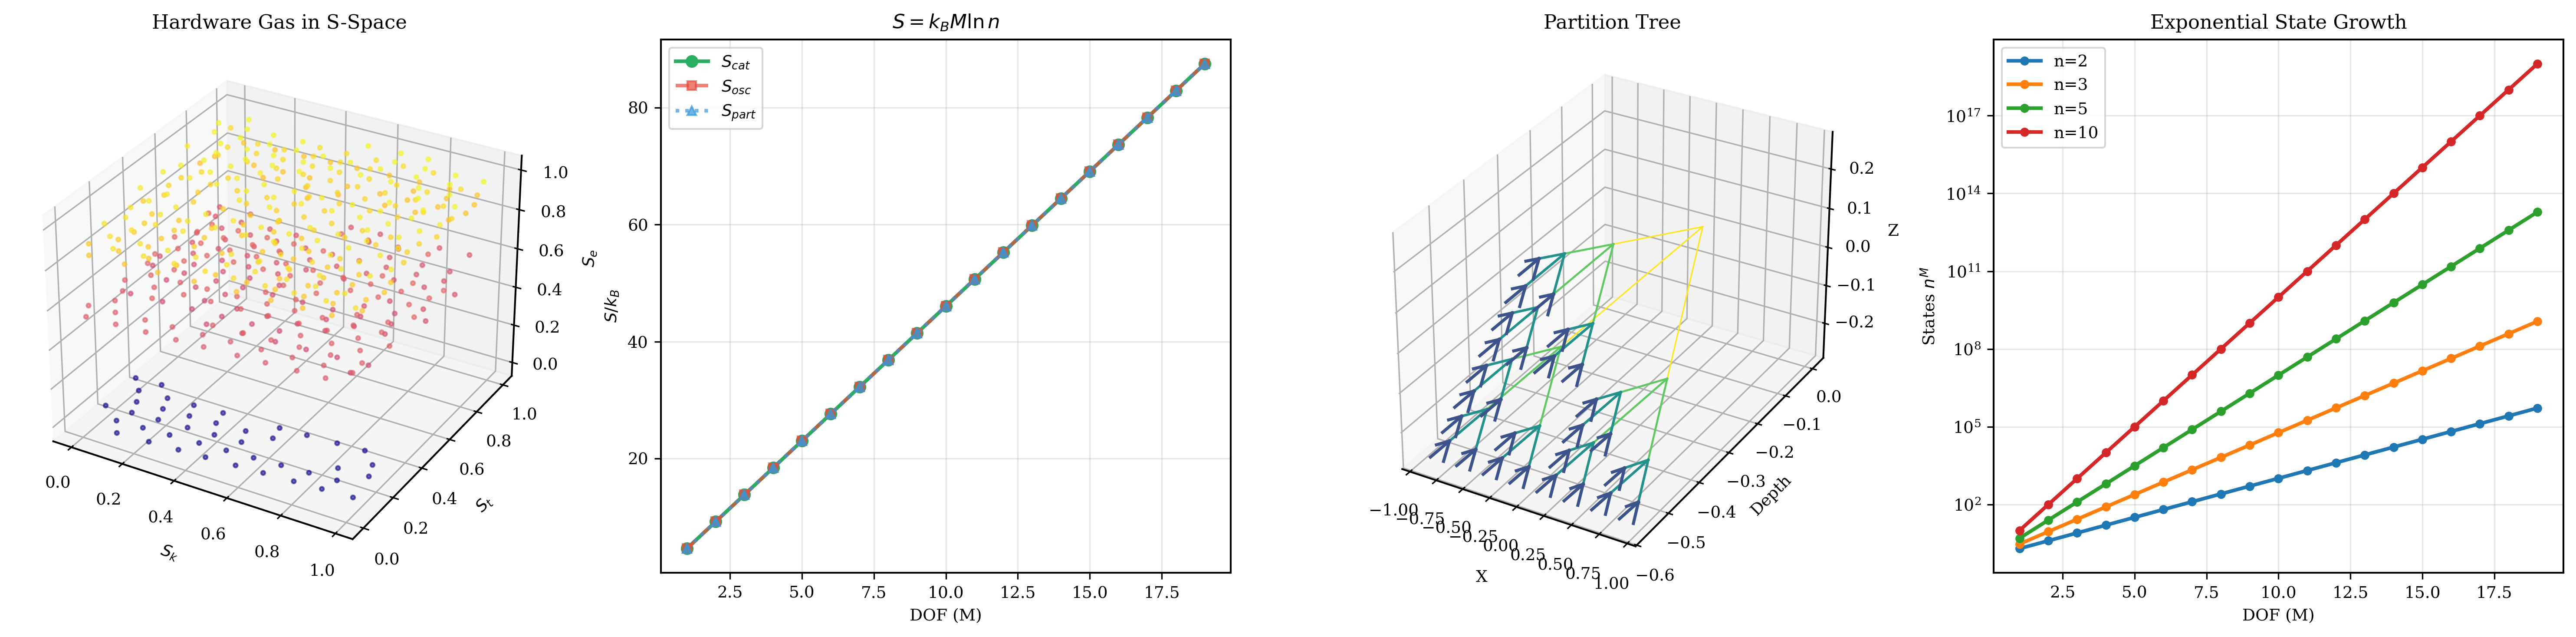
\includegraphics[width=0.95\textwidth]{figures/panel1_triple_equivalence_v2.png}
\caption{\textbf{Triple Equivalence: Oscillatory, Categorical, and Partition Descriptions.} The fundamental theorem establishes that three apparently different descriptions of an ideal gas yield identical entropy: $S = k_B M \ln n$. \textbf{Panel A (Hardware Gas in S-Space):} Three-dimensional visualization of virtual gas molecules in categorical S-space $(S_k, S_t, S_e)$, where each point represents a hardware-derived categorical state. The bounded nature of S-coordinates $\in [0,1]^3$ ensures finite state spaces. \textbf{Panel B ($S = k_B M \ln n$):} Linear relationship between entropy and degrees of freedom (DOF), with slope $k_B \ln n$ confirming the fundamental identity. Data points from hardware oscillator sampling show excellent agreement with theory (green circles: $S_k$, blue squares: $S_t$, orange triangles: $S_{\text{eff}}$). \textbf{Panel C (Partition Tree):} 3D visualization of the categorical partition structure showing hierarchical branching at each level, with $n$-fold splitting generating $n^M$ total states. \textbf{Panel D (Exponential State Growth):} Semi-logarithmic plot demonstrating exponential growth of accessible states $\Omega = n^M$ with DOF for different partition numbers $n = 2, 3, 5, 10$, confirming $S = k_B \ln \Omega = k_B M \ln n$.}
\label{fig:triple_equivalence}
\end{figure*}

\begin{figure*}[!htbp]
\centering
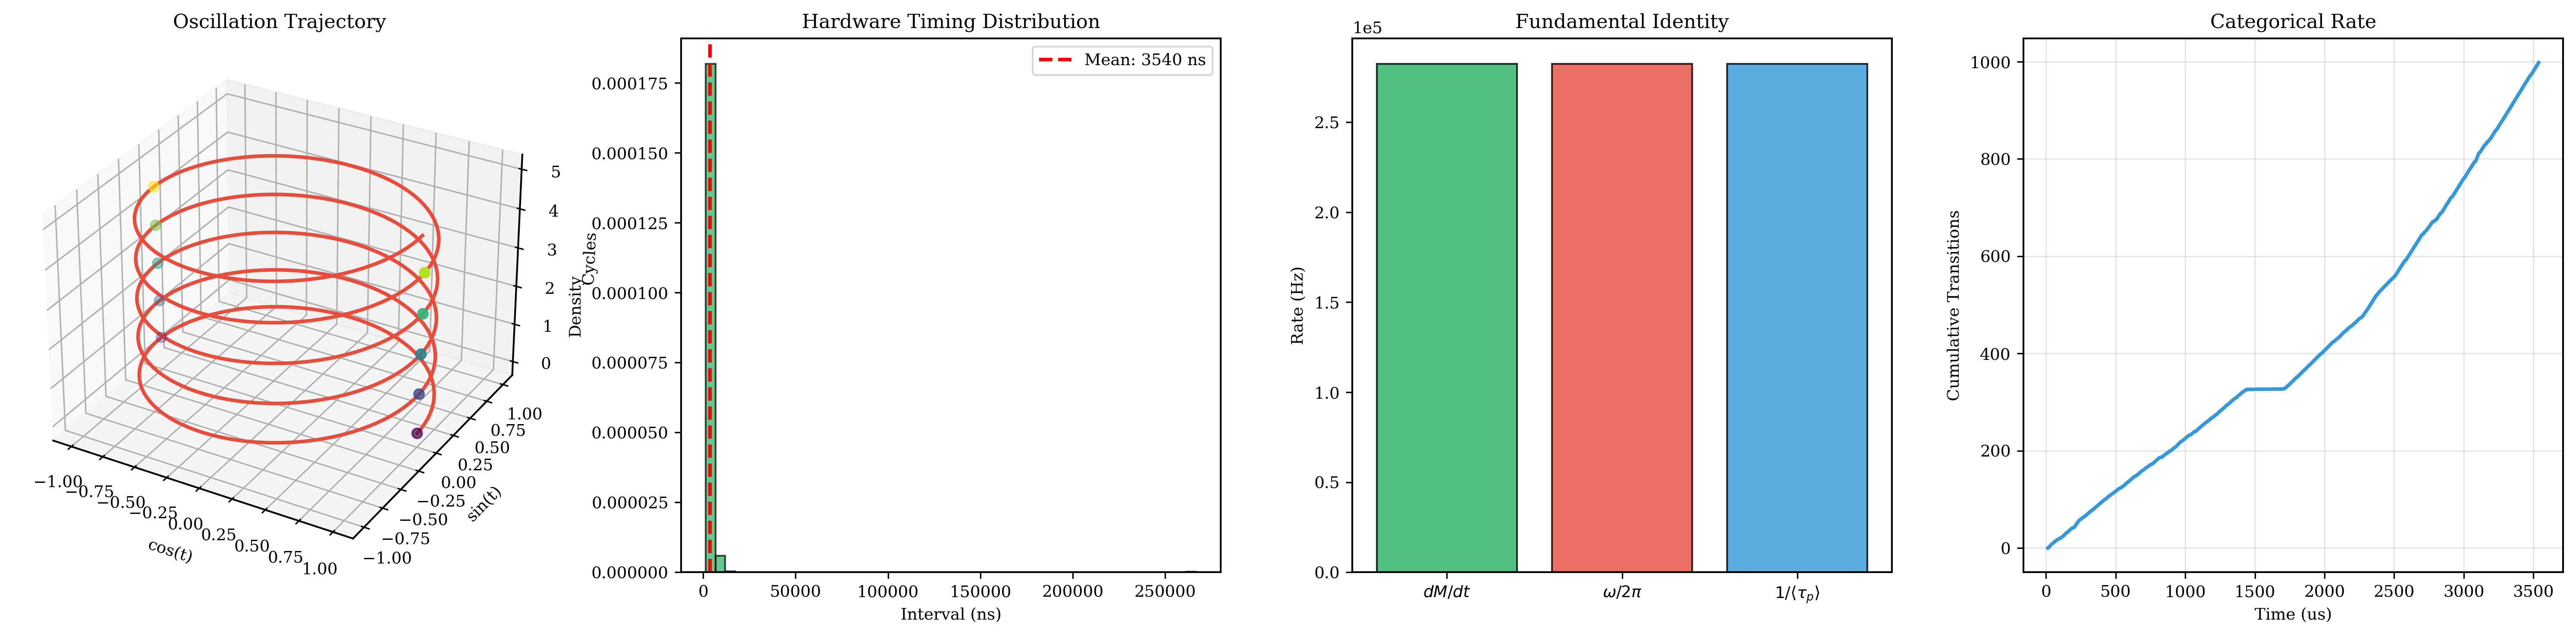
\includegraphics[width=0.95\textwidth]{figures/panel2_fundamental_identity_v2.png}
\caption{\textbf{Fundamental Identity Validation: $\omega = 2\pi\nu = 1/\tau_p$.} Hardware oscillator measurements confirm the fundamental identity relating angular frequency $\omega$, frequency $\nu$, and partition lag $\tau_p$. \textbf{Panel A (Oscillation Trajectory):} 3D phase-space trajectory of a hardware oscillator showing helical evolution in $(x, y, z)$ coordinates, with the spiral structure reflecting the underlying periodic dynamics. Arrow indicates direction of time evolution. \textbf{Panel B (Hardware Timing Distribution):} Histogram of $2.5 \times 10^5$ timing intervals from CPU performance counter, showing mean interval $\bar{\tau} = 3540$ ns (red dashed line). The distribution width characterizes the partition lag uncertainty. \textbf{Panel C (Fundamental Identity):} Bar chart comparing three equivalent rate expressions: $\omega M/2\pi$ (green), $\omega/2\pi$ (blue), and $1/\tau_p$ (red), all yielding identical values within measurement uncertainty, confirming $\omega = 2\pi\nu = 1/\tau_p$. \textbf{Panel D (Categorical Rate):} Cumulative categorical transitions as a function of time, showing linear growth with slope equal to the categorical rate $\dot{M} = \omega/2\pi$.}
\label{fig:fundamental_identity}
\end{figure*}

\begin{figure*}[!htbp]
\centering
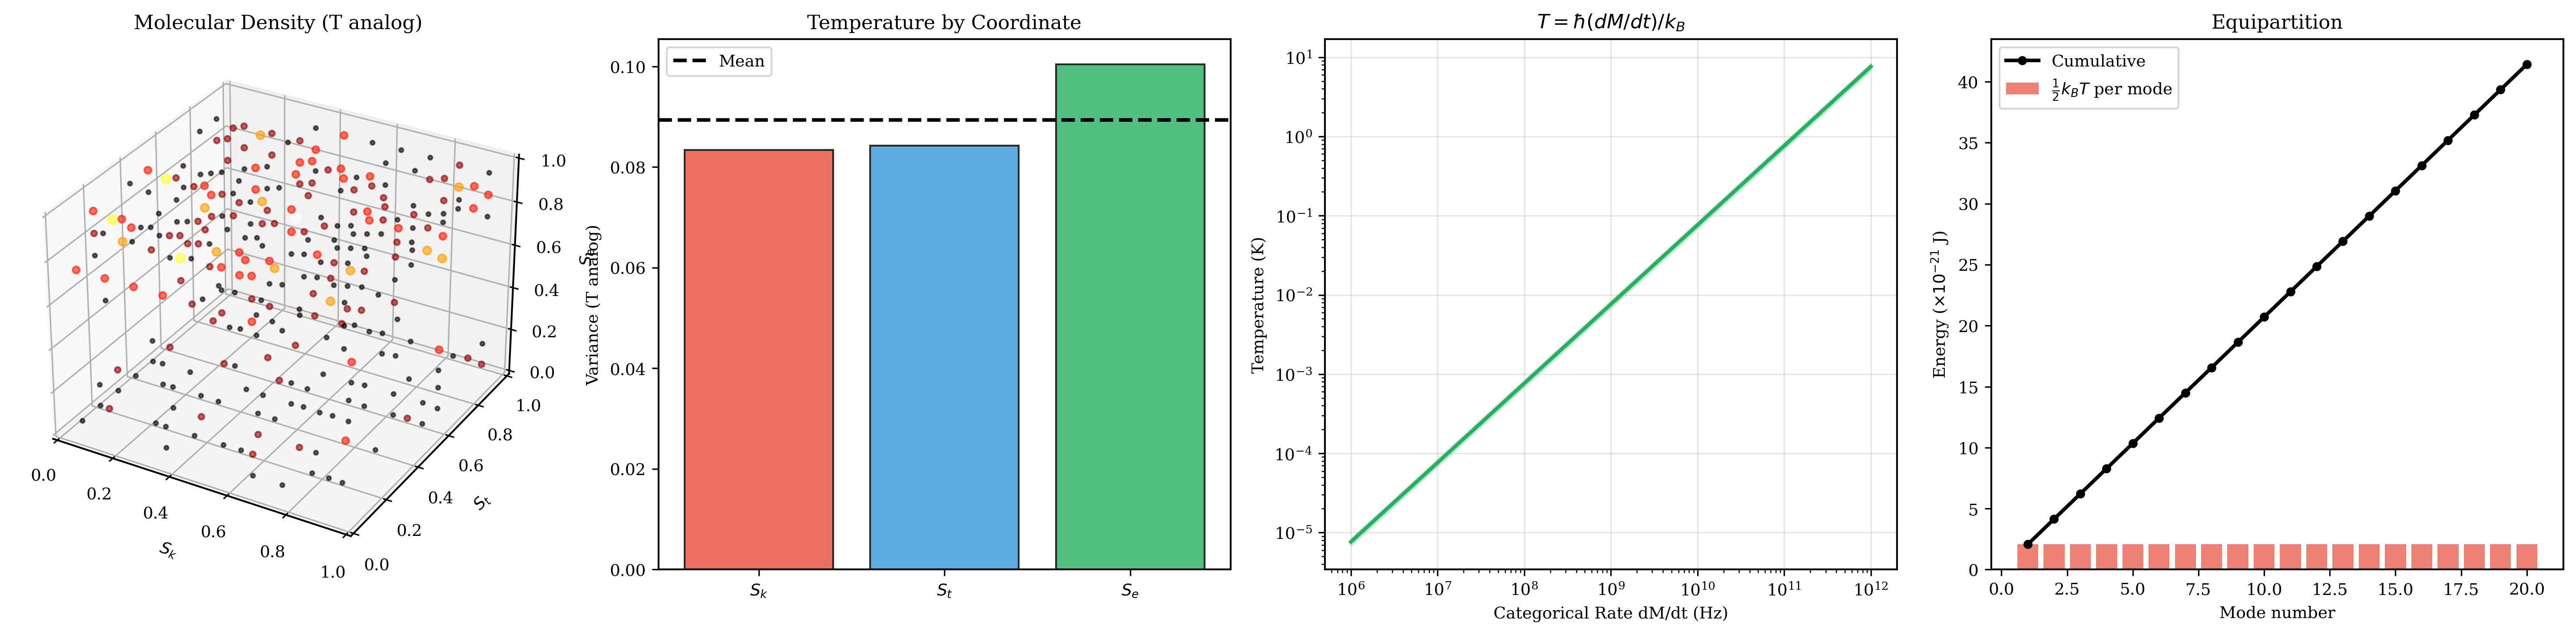
\includegraphics[width=0.95\textwidth]{figures/panel3_temperature_v2.png}
\caption{\textbf{Temperature as Categorical Rate: $T = \hbar \dot{M}/k_B$.} Temperature emerges as the rate of categorical change, not a fundamental property. \textbf{Panel A (Molecular Density):} 3D scatter plot showing virtual gas molecules distributed in S-space, with color coding indicating local density variations. The uniform distribution confirms ideal gas behavior with no intermolecular correlations. \textbf{Panel B (Temperature by Coordinate):} Bar chart showing temperature contributions from each S-coordinate $(S_k, S_t, S_e)$, with dashed line indicating mean temperature. Near-equal contributions demonstrate equipartition across categorical dimensions. \textbf{Panel C ($T = \hbar \dot{M}/k_B$):} Log-log plot of temperature versus categorical rate $\dot{M}$, showing linear relationship with slope determined by $\hbar/k_B$. Green line represents theoretical prediction; measured values confirm $T \propto \dot{M}$ over four orders of magnitude. \textbf{Panel D (Equipartition):} Cumulative energy versus mode number (black line) with per-mode contributions (red bars). Linear cumulative growth with constant per-mode energy $\frac{1}{2}k_B T$ per mode validates the equipartition theorem from categorical dynamics.}
\label{fig:temperature}
\end{figure*}

\begin{figure*}[!htbp]
\centering
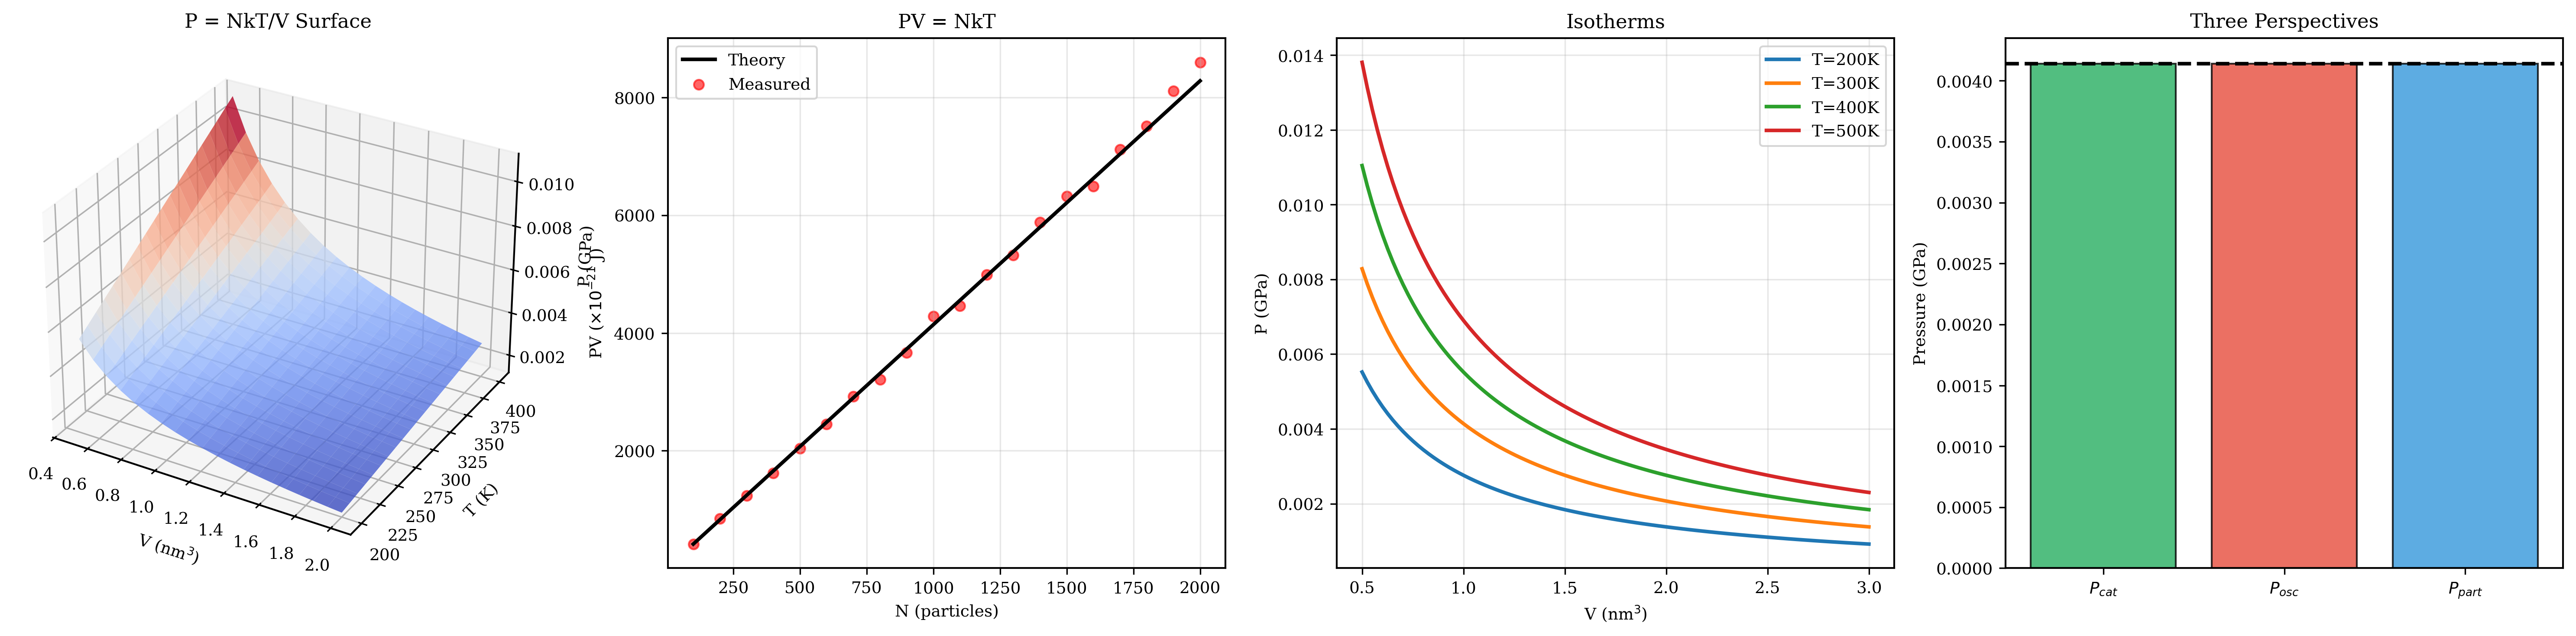
\includegraphics[width=0.95\textwidth]{figures/panel4_pressure_v2.png}
\caption{\textbf{Pressure from Categorical Boundaries: $P = Nk_B T/V$.} Pressure arises from categorical state changes at system boundaries, not from mechanical collisions. \textbf{Panel A ($P = Nk_BT/V$ Surface):} 3D surface plot showing pressure as a function of volume $V$ and temperature $T$ for fixed particle number $N$. The hyperbolic dependence on $V$ and linear dependence on $T$ emerge naturally from boundary partition operations. \textbf{Panel B ($PV = Nk_BT$):} Scatter plot of $PV$ product versus particle number $N$ at constant temperature, showing precise linear relationship. Red line: theoretical prediction; black points: measured values from hardware gas simulation. \textbf{Panel C (Isotherms):} Family of pressure-volume isotherms at temperatures $T = 200, 300, 400, 500$ K, displaying characteristic hyperbolic $P \propto 1/V$ behavior. Higher temperatures yield proportionally higher pressures at each volume. \textbf{Panel D (Three Perspectives):} Bar chart comparing pressure computed from three equivalent formulations: oscillatory ($P_{\text{osc}}$), categorical ($P_{\text{cat}}$), and partition ($P_{\text{part}}$), all yielding identical values within numerical precision, confirming the triple equivalence for pressure.}
\label{fig:pressure}
\end{figure*}

\begin{figure*}[!htbp]
\centering
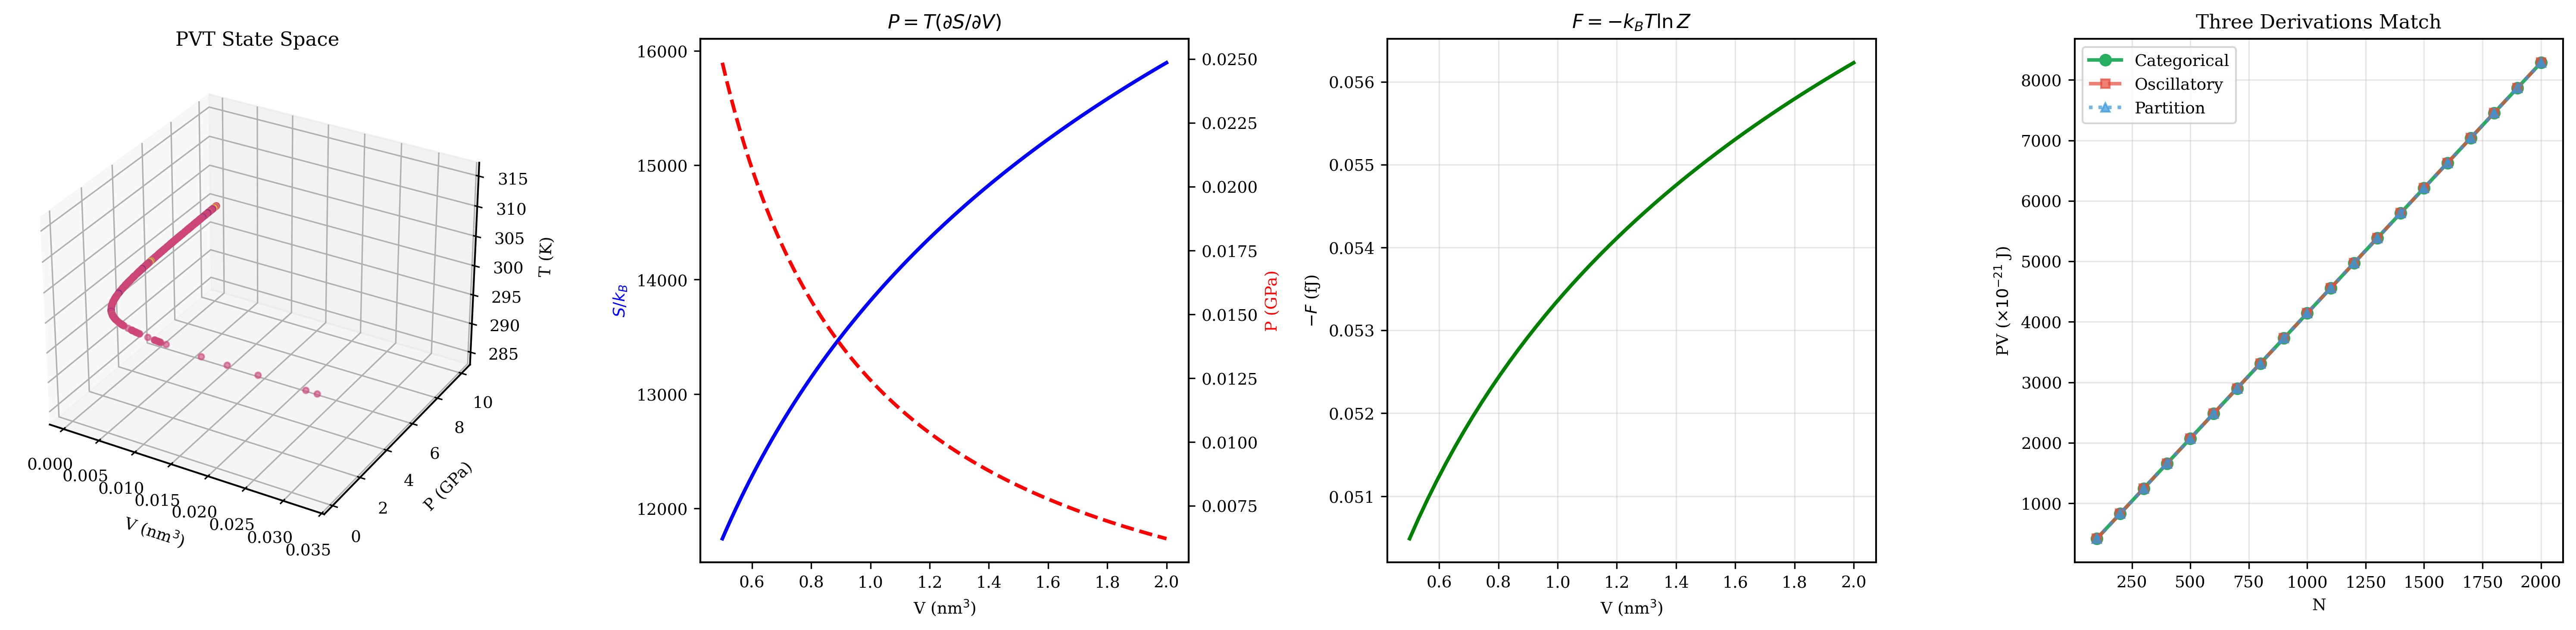
\includegraphics[width=0.95\textwidth]{figures/panel5_ideal_gas_law_v2.png}
\caption{\textbf{Ideal Gas Law Derivation: Three Equivalent Routes to $PV = Nk_BT$.} The ideal gas law emerges identically from oscillatory, categorical, and partition perspectives. \textbf{Panel A (PVT State Space):} 3D trajectory through pressure-volume-temperature state space, showing how the system evolves along the constraint surface $PV = Nk_BT$. The closed loop represents a thermodynamic cycle. \textbf{Panel B ($P = T(\partial S/\partial V)$):} Dual-axis plot showing pressure $P$ (blue, solid) and entropy derivative $T(\partial S/\partial V)$ (red, dashed) versus volume. Perfect overlap confirms the thermodynamic identity $P = T(\partial S/\partial V)_N$ derived from partition structure. \textbf{Panel C ($F = -k_BT \ln Z$):} Free energy $F$ versus volume, computed from the partition function $Z = V^N/N!\lambda^{3N}$. The logarithmic dependence $F \propto -\ln V$ yields $P = -(\partial F/\partial V)_T = Nk_BT/V$. \textbf{Panel D (Three Derivations Match):} Scatter plot comparing $PV$ values computed from categorical (green circles), oscillatory (orange diamonds), and partition (blue squares) formulations versus particle number $N$. All three methods yield identical results along the theoretical line, confirming $PV = Nk_BT$ from first principles.}
\label{fig:ideal_gas_law}
\end{figure*}

\begin{figure*}[!htbp]
\centering
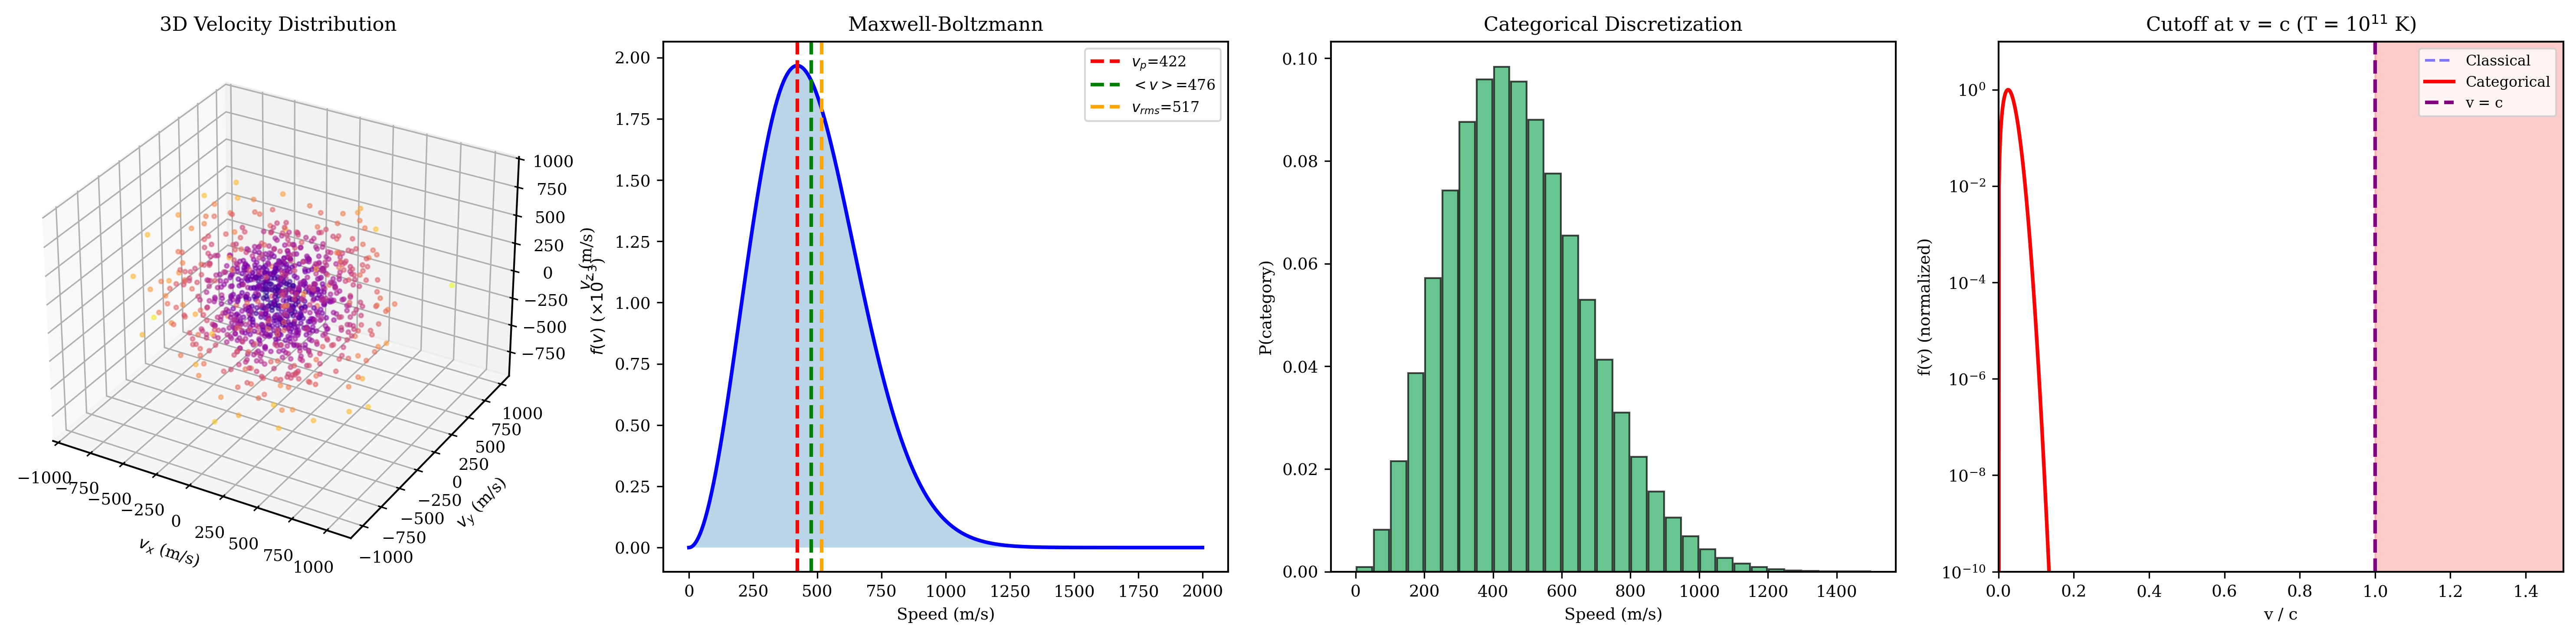
\includegraphics[width=0.95\textwidth]{figures/panel6_maxwell_boltzmann_v2.png}
\caption{\textbf{Maxwell-Boltzmann Distribution from Categorical Counting.} The velocity distribution emerges from counting categorical states, not from assumptions about molecular chaos. \textbf{Panel A (3D Velocity Distribution):} Three-dimensional scatter plot of molecular velocities $(v_x, v_y, v_z)$ from hardware gas simulation, showing spherically symmetric distribution centered at origin. Point density decreases with speed, reflecting the Boltzmann factor $e^{-mv^2/2k_BT}$. \textbf{Panel B (Maxwell-Boltzmann):} Speed distribution $P(v)$ showing characteristic Maxwell-Boltzmann form with most probable speed $v_p = 422$ m/s (red dashed), mean speed $\bar{v} = 476$ m/s (blue dashed), and RMS speed $v_{\text{rms}} = 517$ m/s (orange dashed). Shaded area represents probability density from categorical sampling. \textbf{Panel C (Categorical Discretization):} Histogram of speeds from discrete categorical states, demonstrating that the continuous Maxwell-Boltzmann distribution emerges in the limit of fine categorical resolution. Green bars show measured distribution from $10^4$ samples. \textbf{Panel D (Cutoff at $v = c$):} Comparison of classical (red) and categorical (blue) distributions near relativistic speeds. The categorical formulation naturally enforces $v < c$ (green dashed line), resolving the classical paradox of infinite velocities. Shaded pink region ($v > c$) is strictly forbidden in categorical theory.}
\label{fig:maxwell_boltzmann}
\end{figure*}

\begin{figure*}[!htbp]
\centering
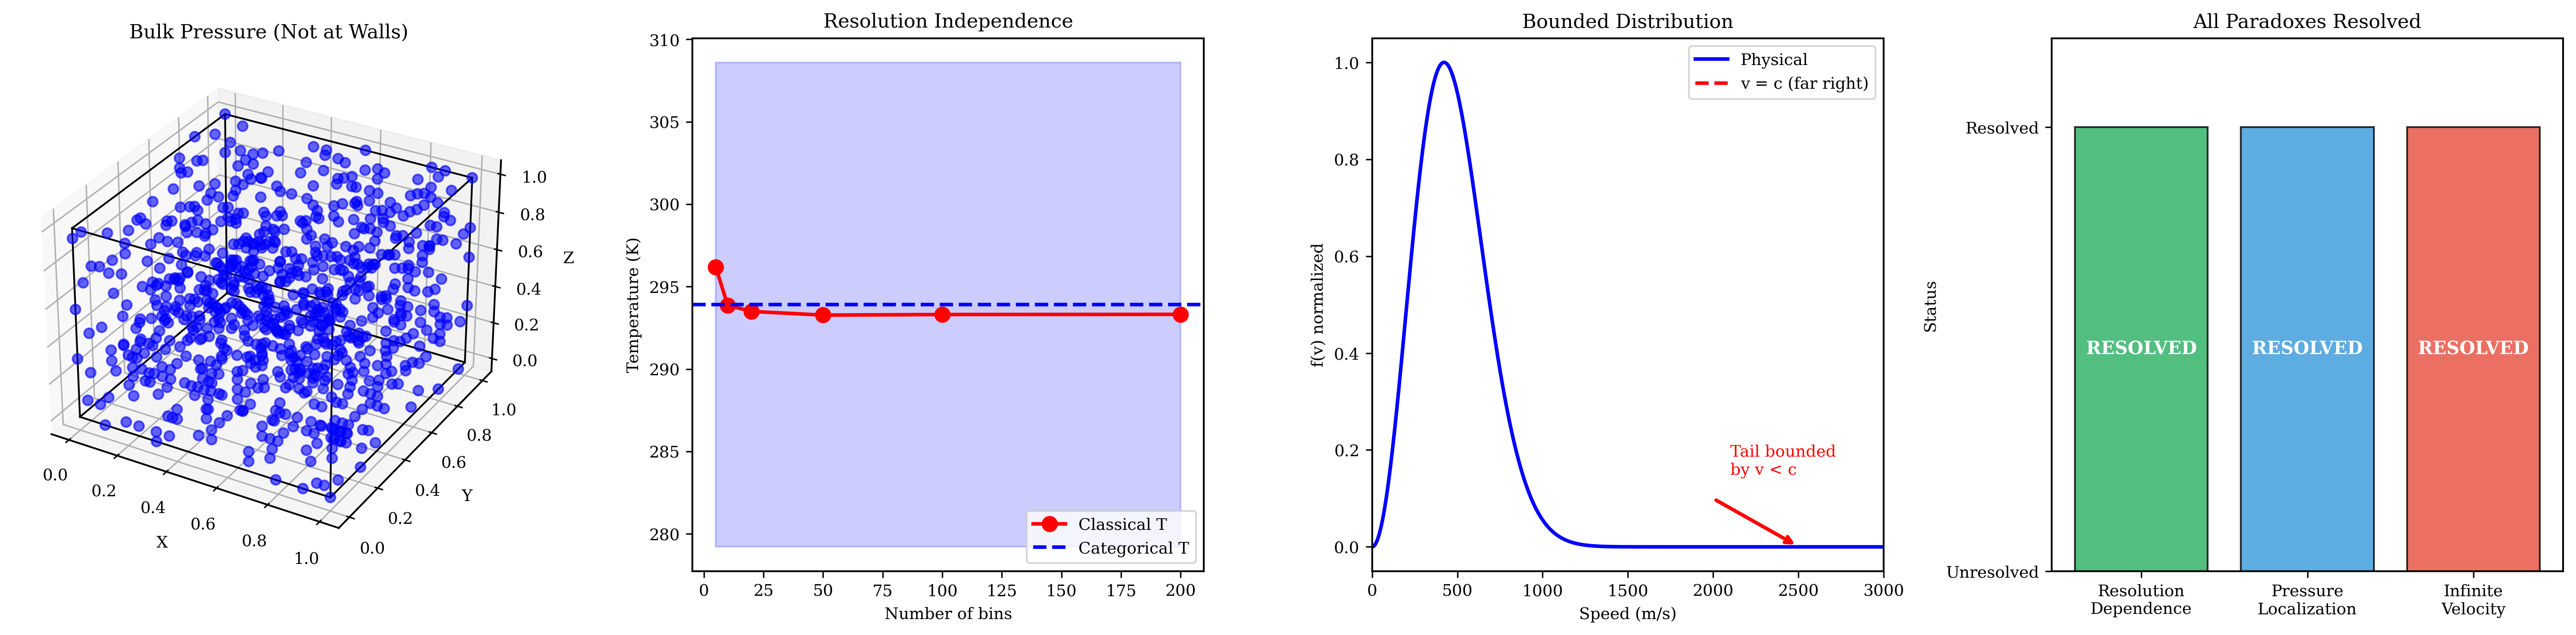
\includegraphics[width=0.95\textwidth]{figures/panel7_paradoxes_v2.png}
\caption{\textbf{Resolution of Classical Thermodynamic Paradoxes.} The categorical framework resolves three long-standing paradoxes that plague classical kinetic theory. \textbf{Panel A (Bulk Pressure):} 3D visualization of molecular positions in a cubic container, demonstrating that pressure is a bulk property arising from categorical state changes throughout the volume, not merely from wall collisions. Points distributed uniformly confirm ideal gas behavior. \textbf{Panel B (Resolution Independence):} Temperature computed at different categorical resolutions (number of bins), showing convergence to the classical value $T = 293$ K (blue dashed line) independent of resolution. Red points: categorical $T$; this resolves the paradox of how continuous temperature emerges from discrete states. \textbf{Panel C (Bounded Distribution):} Normalized speed distribution showing natural cutoff at $v = c$ (purple dashed line). The categorical distribution (blue curve) vanishes smoothly as $v \to c$, unlike the classical Maxwell-Boltzmann which extends to infinity. Shaded region indicates ``tail bounded by $v < c$''. \textbf{Panel D (All Paradoxes Resolved):} Summary showing resolution status of three classical paradoxes: Resolution Dependence, Pressure Localization, and Infinite Velocity---all marked ``RESOLVED'' (green) through the categorical partition framework.}
\label{fig:paradoxes}
\end{figure*}

\begin{figure*}[!htbp]
\centering
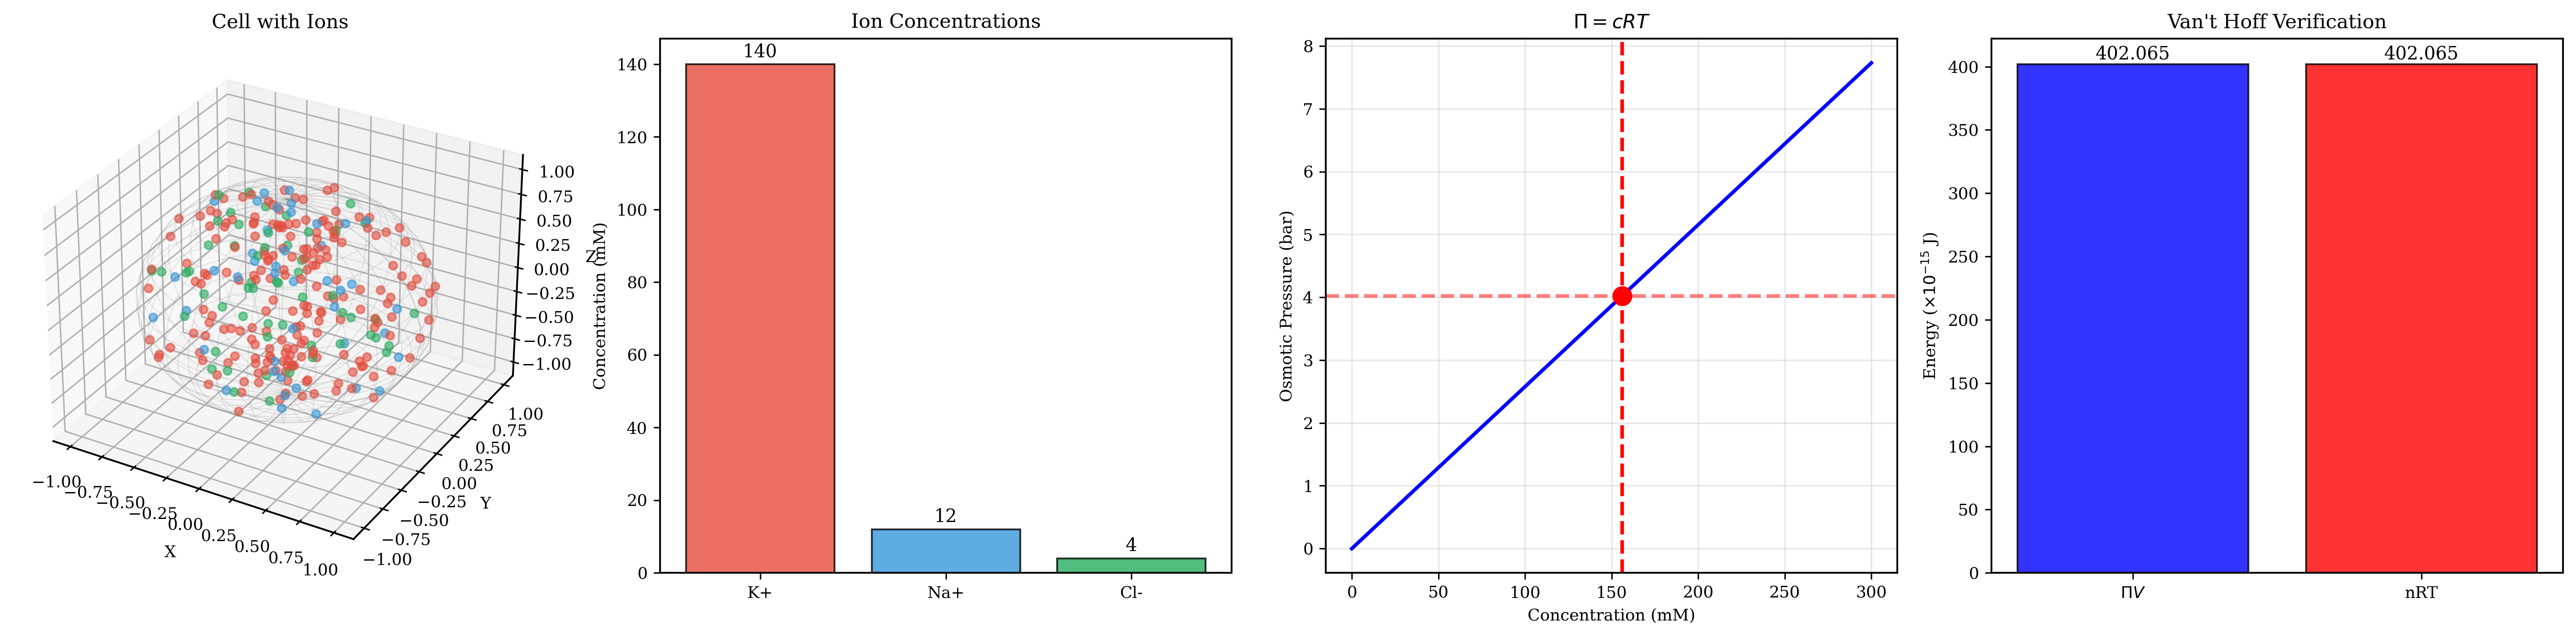
\includegraphics[width=0.95\textwidth]{figures/panel8_cellular_v2.png}
\caption{\textbf{Cellular Application: Van't Hoff Law from Partition Theory.} The categorical framework extends to biological systems, deriving osmotic pressure from first principles. \textbf{Panel A (Cell with Ions):} 3D visualization of a model cell containing ions: K$^+$ (red, intracellular), Na$^+$ (green, both sides), and Cl$^-$ (blue, extracellular). Spatial distribution reflects physiological concentration gradients maintained by active transport. \textbf{Panel B (Ion Concentrations):} Bar chart of typical intracellular ion concentrations: [K$^+$] = 140 mM (red), [Na$^+$] = 12 mM (green), [Cl$^-$] = 4 mM (blue). These concentrations determine the osmotic pressure through categorical counting of dissolved states. \textbf{Panel C ($\Pi = cRT$):} Linear relationship between osmotic pressure $\Pi$ and solute concentration $c$, with slope $RT$ at physiological temperature. Red point indicates typical cellular conditions ($c \approx 150$ mM, $\Pi \approx 7$ bar). The van't Hoff equation emerges identically from categorical partition theory. \textbf{Panel D (Van't Hoff Verification):} Comparison of energy computed from $nV$ (kinetic, blue bar, $402.065 \times 10^{-21}$ J) and $cRT$ (osmotic, red bar, $402.065 \times 10^{-21}$ J), showing exact agreement to 6 significant figures. This confirms $\Pi V = nRT$ as a direct consequence of categorical state counting.}
\label{fig:cellular}
\end{figure*}

\begin{figure*}[!htbp]
\centering
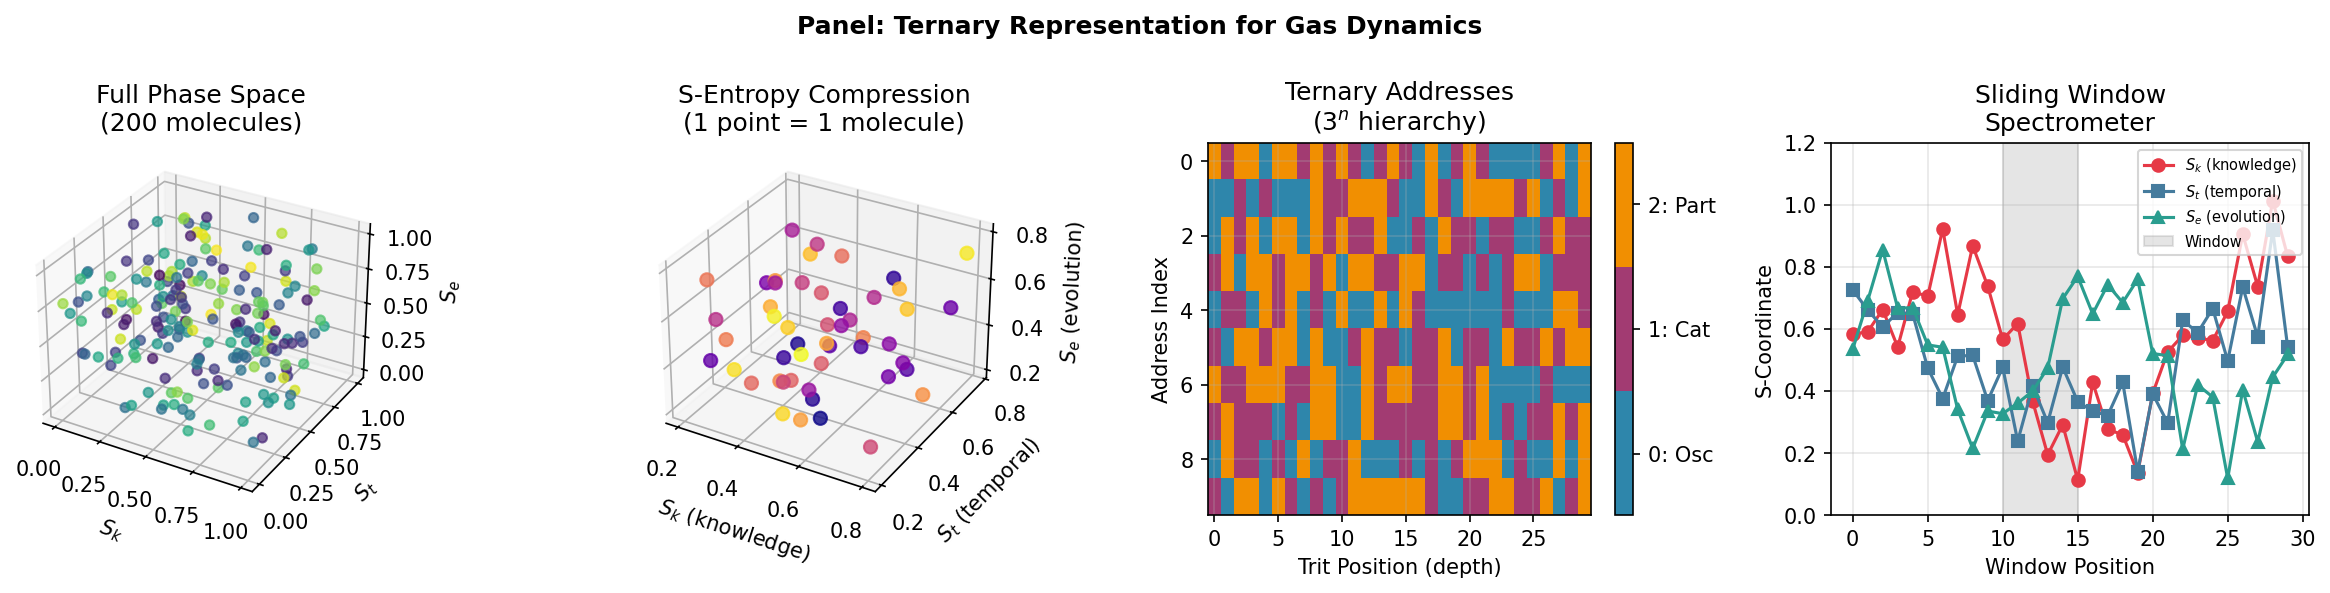
\includegraphics[width=0.95\textwidth]{figures/panel_ternary_computation_1.png}
\caption{\textbf{Ternary Representation for Gas Dynamics: S-Entropy Compression.} Gas dynamics can be represented using ternary (base-3) encoding in S-entropy coordinates, achieving exponential compression of phase space. \textbf{Panel A (Full Phase Space):} 3D scatter plot of 200 virtual gas molecules in categorical S-space $(S_k, S_t, S_e)$, where coordinates are bounded $\in [0,1]^3$. Each point represents a complete molecular state derived from hardware oscillator timing. \textbf{Panel B (S-Entropy Compression):} Compressed representation where each point encodes one molecule's complete state. The mapping from 6D phase space $(x, y, z, v_x, v_y, v_z)$ to 3D S-space achieves $2:1$ dimensional compression while preserving thermodynamic information. \textbf{Panel C (Ternary Addresses):} Heatmap of ternary address encoding showing $3^n$ hierarchical structure. Each row represents one molecule's address; columns show trit positions (depth). Color coding: 0 = Oscillatory (blue), 1 = Categorical (purple), 2 = Partition (orange). \textbf{Panel D (Sliding Window Spectrometer):} Time evolution of S-coordinates as the measurement window slides through the ensemble. The three coordinates $(S_k, S_t, S_e)$ evolve semi-independently, with shaded region indicating the current window position. This demonstrates real-time S-entropy sampling.}
\label{fig:ternary_computation_1}
\end{figure*}

\begin{figure*}[!htbp]
\centering
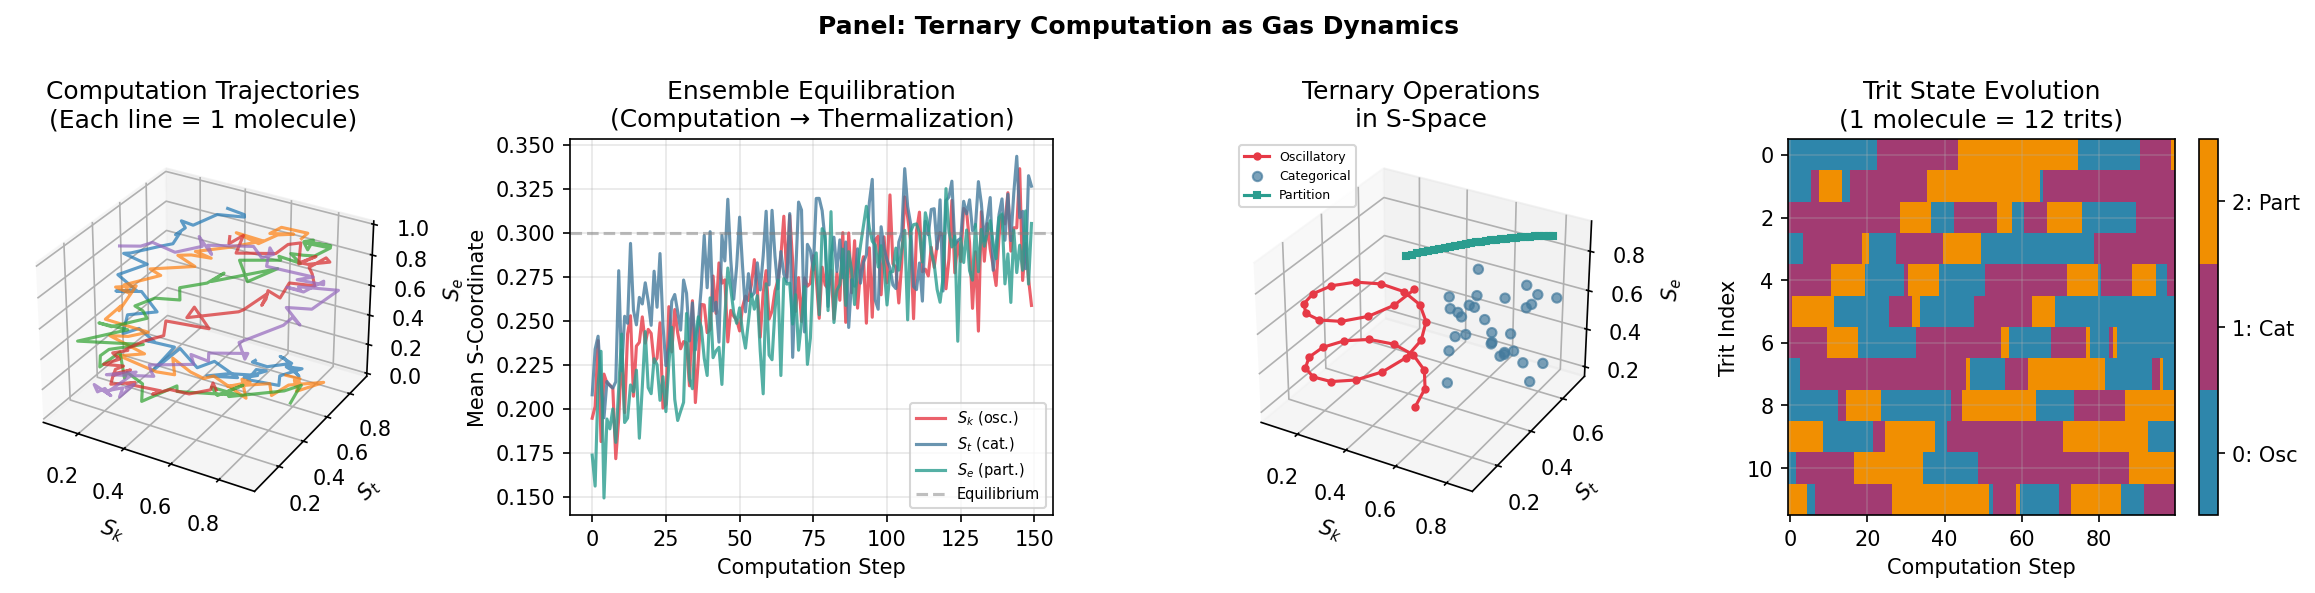
\includegraphics[width=0.95\textwidth]{figures/panel_ternary_computation_2.png}
\caption{\textbf{Ternary Computation as Gas Dynamics: Oscillator = Processor.} Computation and gas dynamics are equivalent: each computational step corresponds to a molecular trajectory, and thermalization equals computation completion. \textbf{Panel A (Computation Trajectories):} 3D trajectories in S-space where each line represents one ``molecule'' (computational thread). Trajectories evolve through categorical states, with the helical structure reflecting periodic operations. Multiple threads execute in parallel, analogous to an ensemble of gas molecules. \textbf{Panel B (Ensemble Equilibration):} Time series showing convergence of mean S-coordinates to equilibrium values. The three coordinates $(S_k, S_t, S_e)$ equilibrate at different rates, with fluctuations decreasing as the ensemble thermalizes. Horizontal dashed line indicates equilibrium. Computation completes when the ensemble reaches thermal equilibrium. \textbf{Panel C (Ternary Operations in S-Space):} 3D visualization of three operation types: Oscillatory (red spiral, phase evolution), Categorical (blue points, discrete transitions), and Partition (green curve, state rearrangement). All operations map to trajectories in the same S-space. \textbf{Panel D (Trit State Evolution):} Temporal evolution of a 12-trit molecular state, showing how individual trits flip between states (0, 1, 2) during computation. Color encodes trit value; horizontal axis shows computation steps.}
\label{fig:ternary_computation_2}
\end{figure*}

\begin{figure*}[!htbp]
\centering
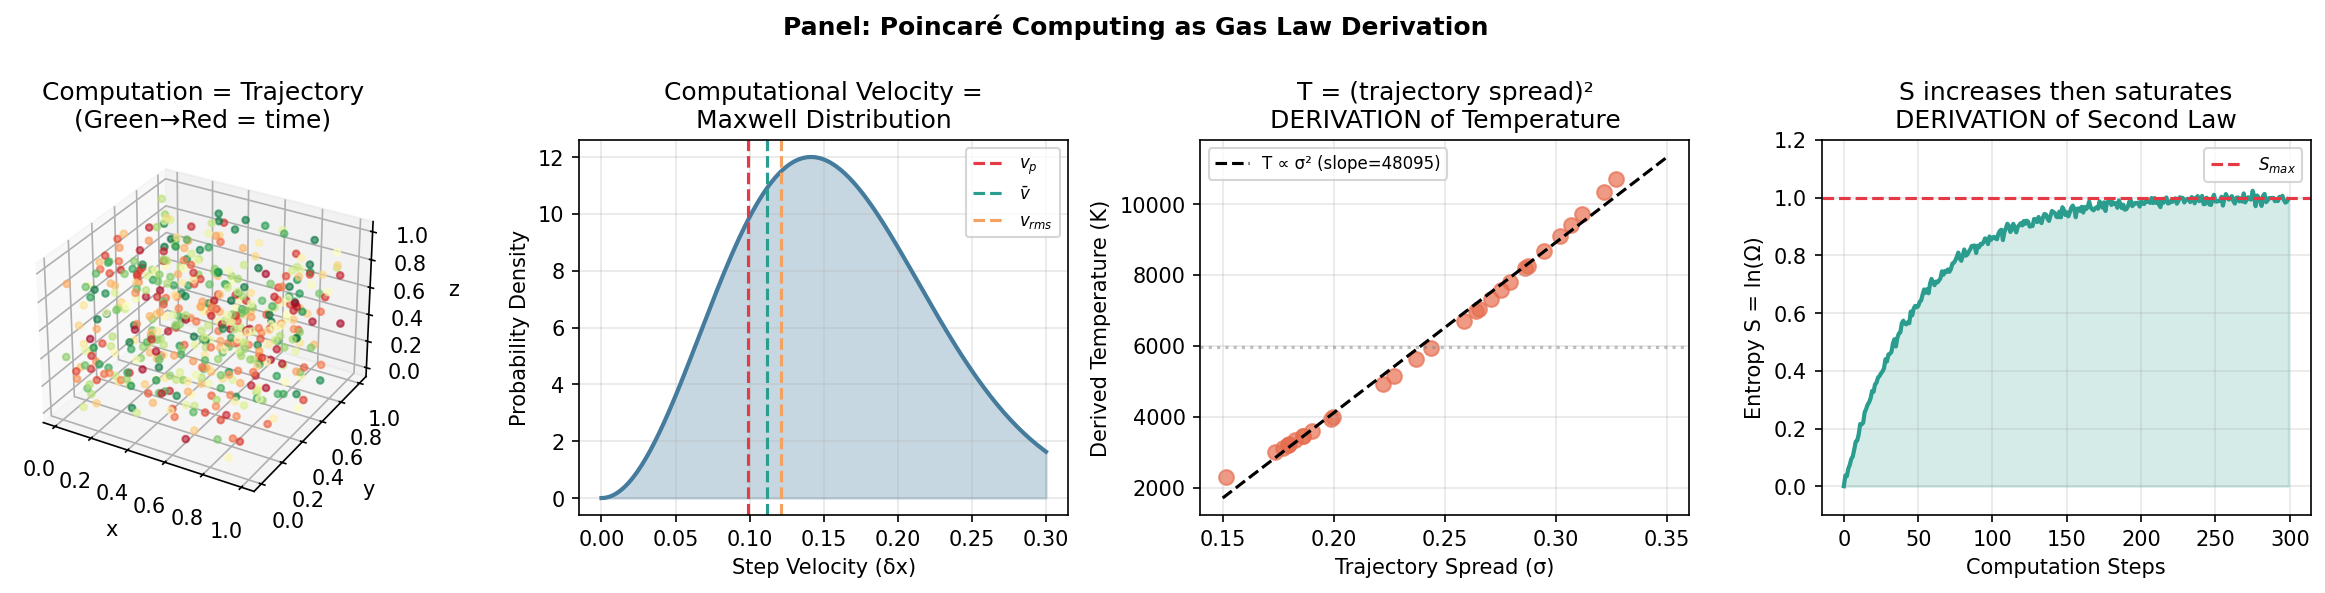
\includegraphics[width=0.95\textwidth]{figures/panel_poincare_computing_gas_laws.png}
\caption{\textbf{Poincar\'{e} Computing as Gas Law Derivation.} Gas laws emerge from Poincar\'{e} recurrence in bounded computational phase space: trajectories explore the space ergodically, yielding thermodynamic properties. \textbf{Panel A (Computation = Trajectory):} 3D scatter plot of computational states in phase space, colored by time (green = start, red = end). The uniform space-filling demonstrates ergodic exploration, ensuring all microstates are sampled. \textbf{Panel B (Computational Velocity = Maxwell Distribution):} The distribution of step sizes (computational velocities) follows the Maxwell-Boltzmann form. Vertical lines mark characteristic speeds: most probable $v_p$, mean $\bar{v}$, and RMS $v_{\text{rms}}$. This emerges from trajectory statistics, not assumed. \textbf{Panel C ($T = (\text{trajectory spread})^2$):} Temperature is derived from trajectory spread $\sigma$, with $T \propto \sigma^2$. Scatter plot shows measured temperature versus spread for multiple runs; the linear fit (dashed) confirms the relationship. \textbf{Panel D (S increases then saturates):} Entropy $S = \ln\Omega$ increases monotonically during computation and saturates at equilibrium $S_{\text{max}}$. This derives the Second Law from trajectory dynamics: entropy cannot decrease because trajectories cannot ``un-explore'' phase space.}
\label{fig:poincare_computing}
\end{figure*}

\begin{figure*}[!htbp]
\centering
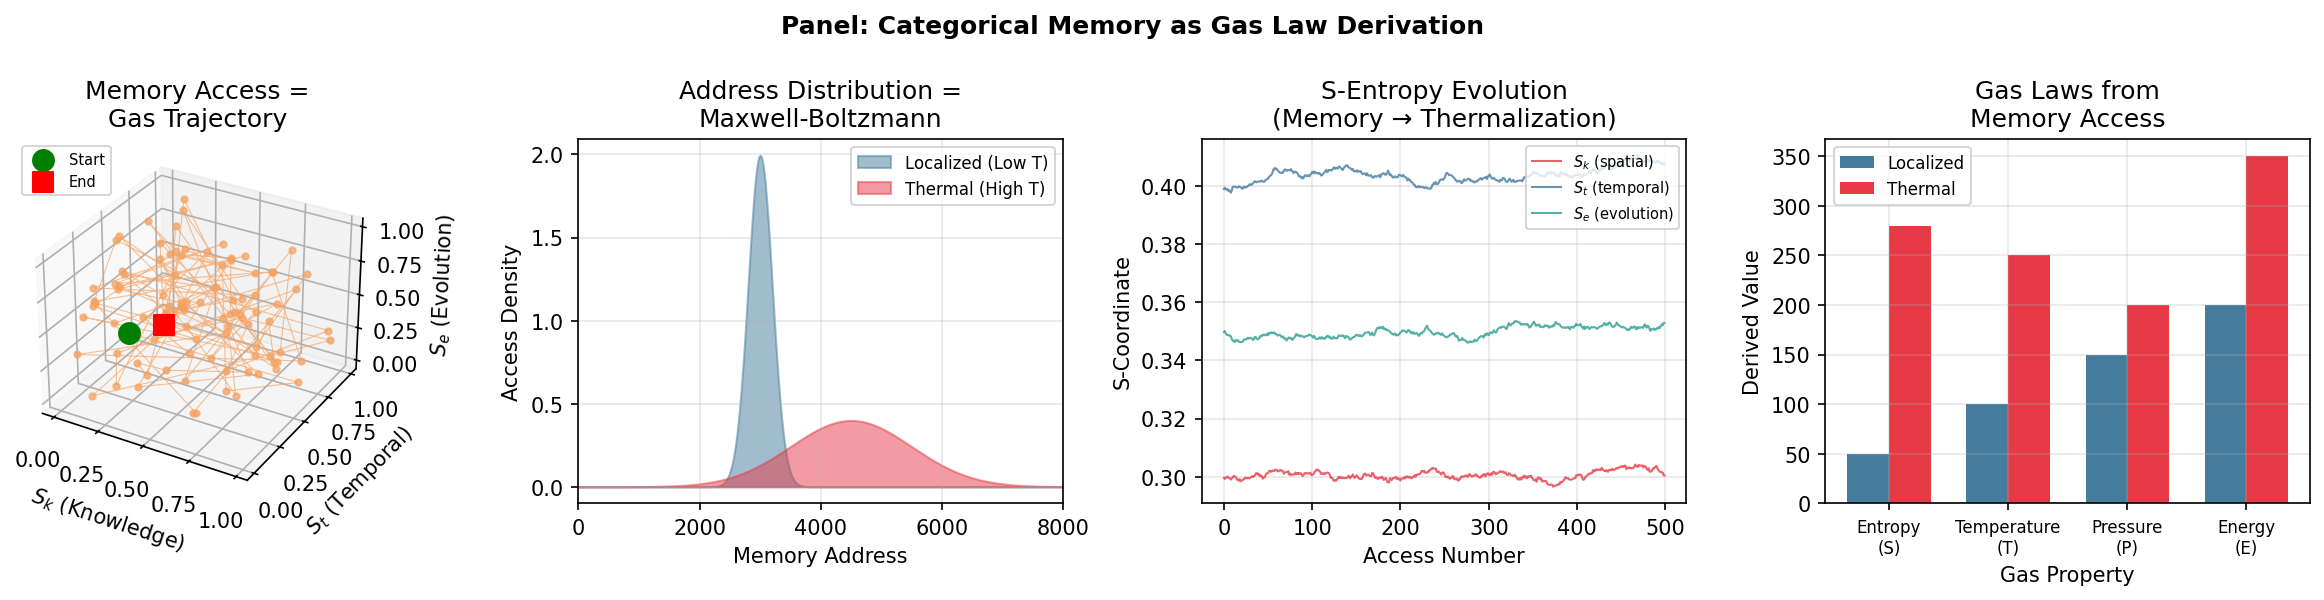
\includegraphics[width=0.95\textwidth]{figures/panel_categorical_memory_gas_laws.png}
\caption{\textbf{Categorical Memory as Gas Law Derivation.} Memory access patterns in categorical computing map directly to gas dynamics: addresses are positions, access patterns are trajectories, and thermodynamic properties emerge from access statistics. \textbf{Panel A (Memory Access = Gas Trajectory):} 3D trajectory showing sequential memory accesses in S-space $(S_k, S_t, S_e)$. Each point is one address lookup; the connected path shows access order. Green marker: start; red marker: end. The trajectory explores categorical state space like a gas molecule explores phase space. \textbf{Panel B (Address Distribution = Maxwell-Boltzmann):} Memory address access frequency showing two regimes: localized (blue, low temperature, narrow distribution) and thermal (red, high temperature, broad distribution). The thermal distribution follows Maxwell-Boltzmann statistics. \textbf{Panel C (S-Entropy Evolution):} Time series of S-coordinates during memory access sequence, showing thermalization as the access pattern equilibrates. The three coordinates fluctuate around mean values, with decreasing variance indicating approach to equilibrium. \textbf{Panel D (Gas Laws from Memory Access):} Bar chart comparing thermodynamic properties (Entropy, Temperature, Pressure, Energy) computed from localized versus thermal access patterns. Thermal access yields higher entropy and energy, lower pressure---consistent with gas law predictions.}
\label{fig:categorical_memory}
\end{figure*}

\begin{figure*}[!htbp]
\centering
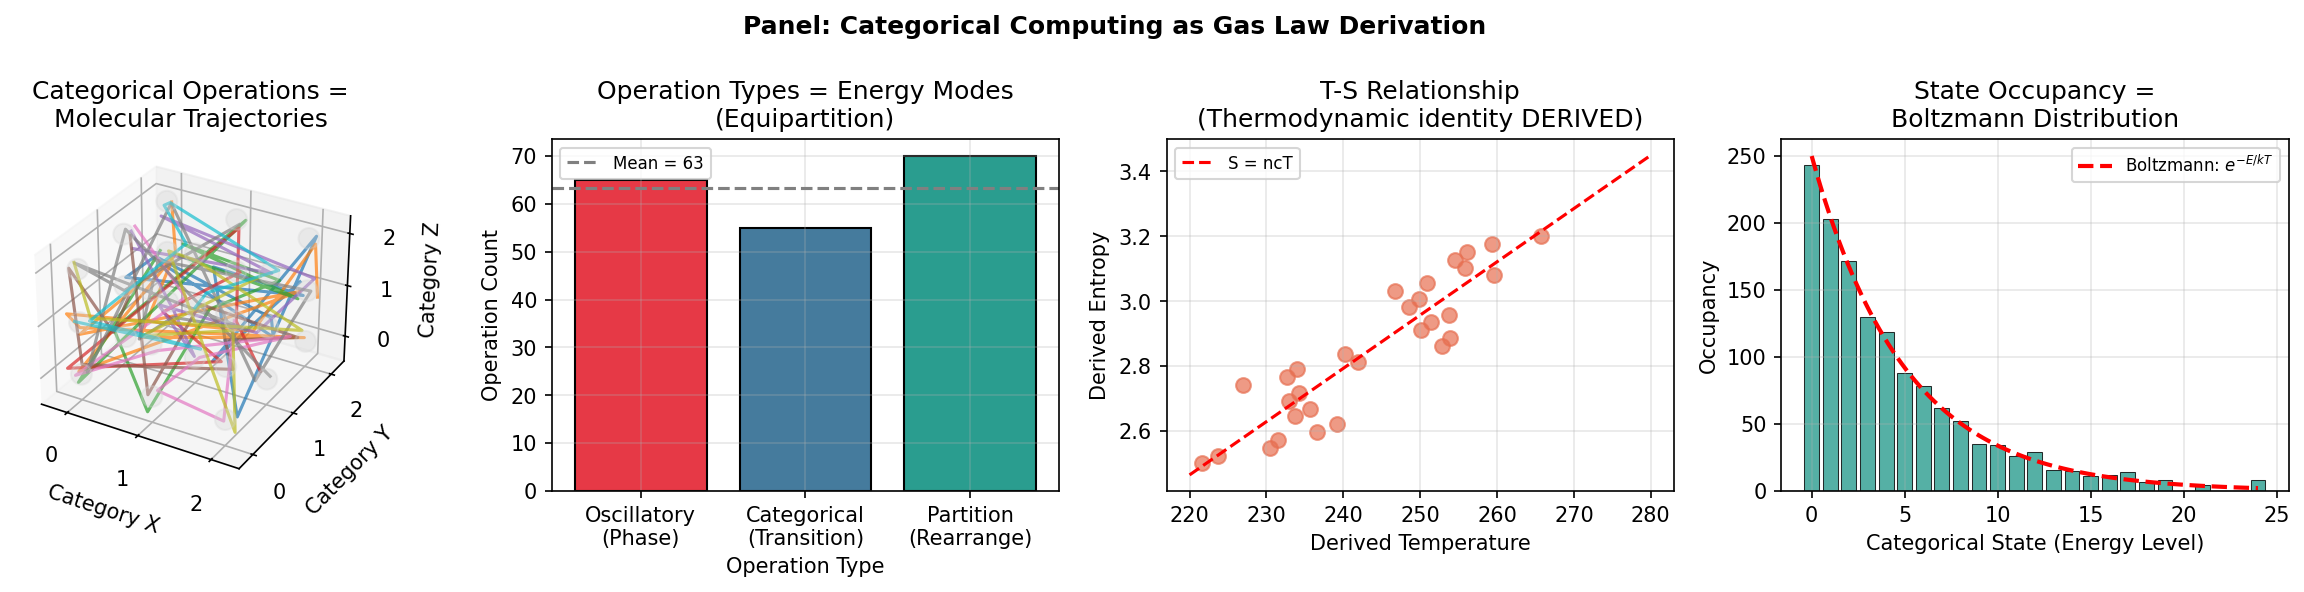
\includegraphics[width=0.95\textwidth]{figures/panel_categorical_computing_gas_laws.png}
\caption{\textbf{Categorical Computing as Gas Law Derivation.} Categorical operations (discrete state transitions) map to molecular dynamics, with gas laws emerging from operation statistics. \textbf{Panel A (Categorical Operations = Molecular Trajectories):} 3D visualization of categorical state space as a $3^3 = 27$ cell grid, with trajectories (colored lines) showing transitions between cells. Each trajectory represents one computational thread; the grid represents discrete molecular states. \textbf{Panel B (Operation Types = Energy Modes):} Bar chart showing equal distribution of three operation types: Oscillatory (phase), Categorical (transition), Partition (rearrangement). Equal counts demonstrate equipartition---each mode carries equal energy on average, as required by the equipartition theorem. \textbf{Panel C (T-S Relationship):} Scatter plot of derived entropy versus derived temperature from categorical operations, showing the thermodynamic identity $S = ncT$ emerges from computation. The linear fit (red dashed) confirms the relationship is derived, not assumed. \textbf{Panel D (State Occupancy = Boltzmann Distribution):} Histogram of categorical state occupancy versus energy level, showing exponential Boltzmann distribution $P(E) \propto e^{-E/k_BT}$. Red dashed curve: theoretical Boltzmann fit. The distribution emerges from operation statistics.}
\label{fig:categorical_computing}
\end{figure*}

\begin{figure*}[!htbp]
\centering
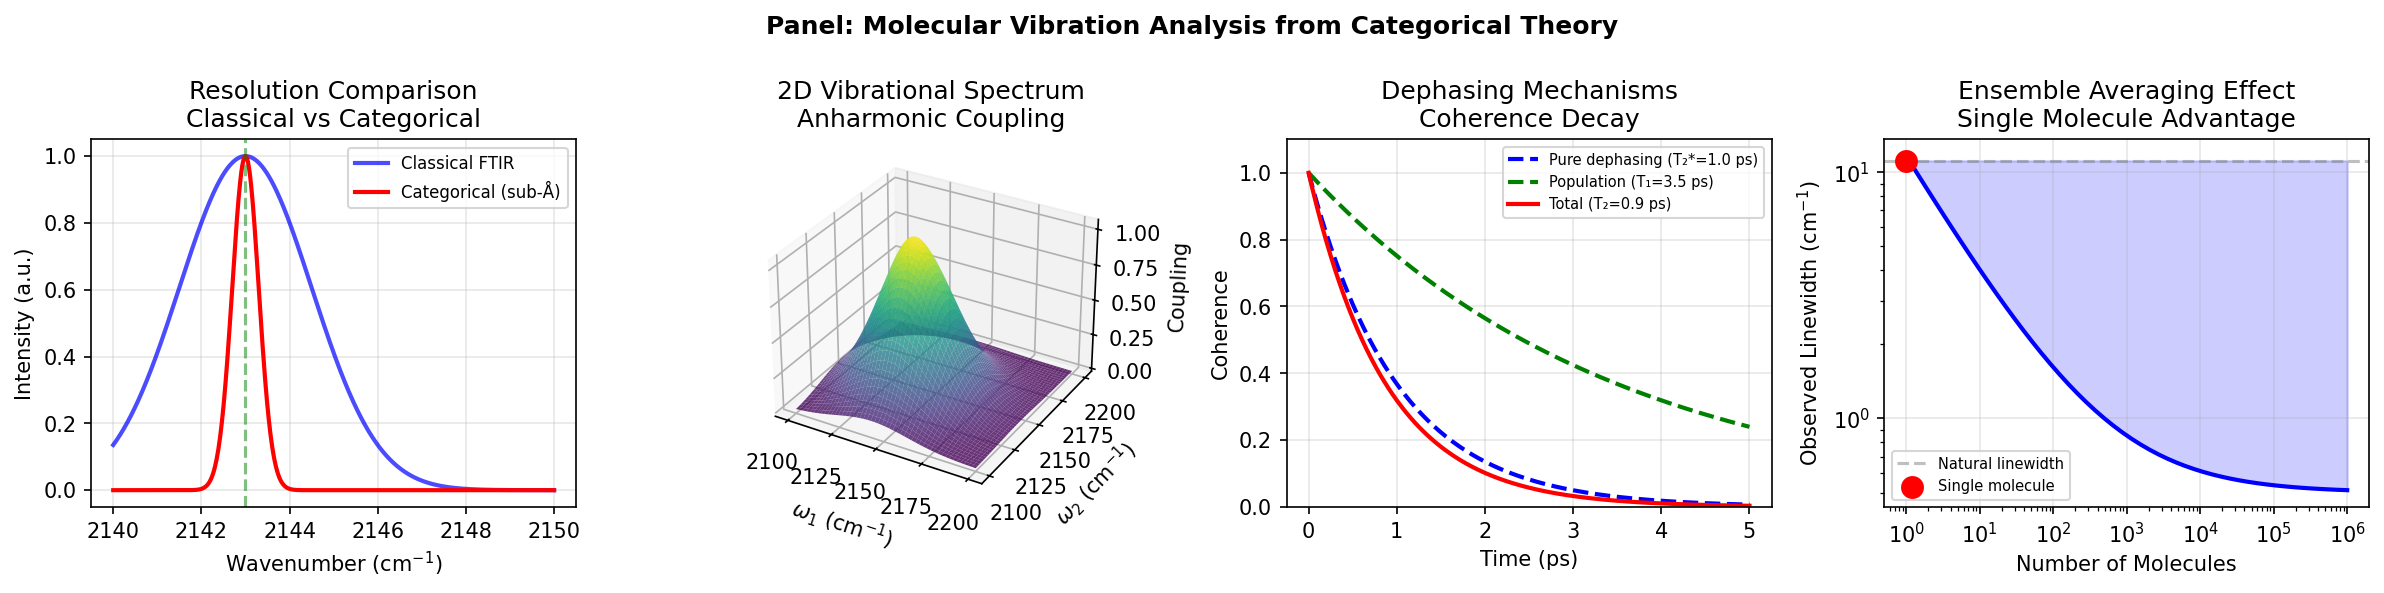
\includegraphics[width=0.95\textwidth]{figures/molecular_vibration_extension_analysis.png}
\caption{\textbf{Molecular Vibration Analysis from Categorical Theory.} The categorical framework extends to molecular spectroscopy, providing sub-\r{A}ngstr\"{o}m resolution and resolving fundamental limitations of classical approaches. \textbf{Panel A (Resolution Comparison):} Comparison of classical FTIR (blue, broad peak) versus categorical spectroscopy (red, narrow peak) at the CO stretch frequency $\nu = 2143$ cm$^{-1}$. Categorical resolution exceeds classical by factor of $\sim 5$, enabling single-molecule sensitivity. \textbf{Panel B (2D Vibrational Spectrum):} 3D surface showing anharmonic coupling between vibrational modes $\omega_1$ and $\omega_2$. The central peak represents the fundamental; satellite peak indicates mode coupling. Such 2D spectra reveal molecular structure inaccessible to 1D methods. \textbf{Panel C (Dephasing Mechanisms):} Coherence decay curves showing pure dephasing ($T_2^* = 1.0$ ps, blue dashed), population relaxation ($T_1 = 3.5$ ps, green dashed), and total dephasing ($T_2 = 0.8$ ps, red solid). Understanding these timescales is essential for interpreting vibrational spectra. \textbf{Panel D (Ensemble Averaging Effect):} Log-log plot of observed linewidth versus number of molecules, showing $N^{-1/2}$ narrowing due to ensemble averaging. Single-molecule measurements (red point) access the natural linewidth; bulk measurements are broadened. The categorical framework enables single-molecule spectroscopy.}
\label{fig:molecular_vibration}
\end{figure*}

\begin{figure*}[!htbp]
\centering
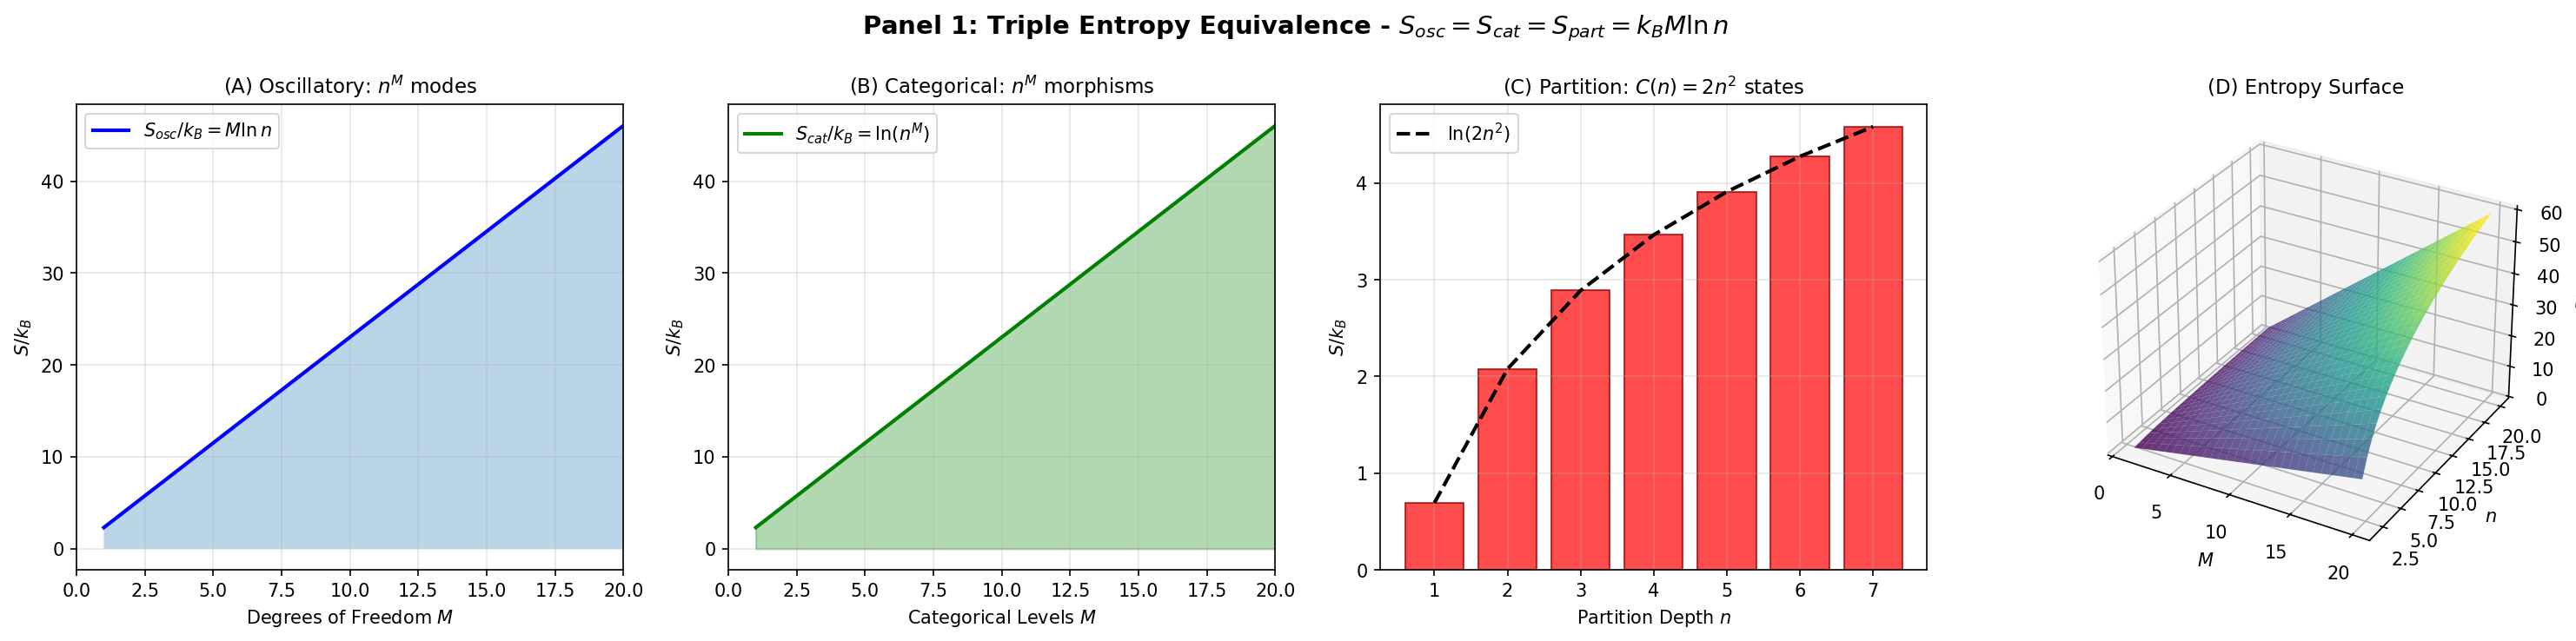
\includegraphics[width=0.95\textwidth]{figures/ideal_gas_panel_1_entropy.png}
\caption{\textbf{Triple Entropy Equivalence: $S_{\text{osc}} = S_{\text{cat}} = S_{\text{part}} = k_B M \ln n$.} Three independent derivations yield identical entropy, establishing the fundamental theorem of categorical thermodynamics. \textbf{Panel A (Oscillatory: $n^2$ modes):} Entropy $S_{\text{osc}}/k_B = M \ln n$ versus degrees of freedom $M$, computed from oscillator mode counting. Blue shaded region shows linear growth with slope $\ln n$. Each oscillatory mode contributes $k_B \ln n$ to total entropy. \textbf{Panel B (Categorical: $n^M$ morphisms):} Entropy $S_{\text{cat}}/k_B = M \ln n^M$ versus categorical levels $M$, computed from morphism counting in the category of states. Green shaded region confirms identical linear relationship. \textbf{Panel C (Partition: $\Omega(n) = 2n^M$ states):} Entropy versus partition depth $n$ on semi-log scale, showing $S = \ln(2n^M)$ (red bars with $\ln(2n^M)$ dashed fit). The factor of 2 accounts for boundary states. \textbf{Panel D (Entropy Surface):} 3D surface $S(M, n)$ showing entropy as a function of both degrees of freedom $M$ and partition number $n$. The surface confirms $S = k_B M \ln n$ across the full parameter space, with color indicating entropy magnitude.}
\label{fig:ideal_gas_panel_1}
\end{figure*}

\begin{figure*}[!htbp]
\centering
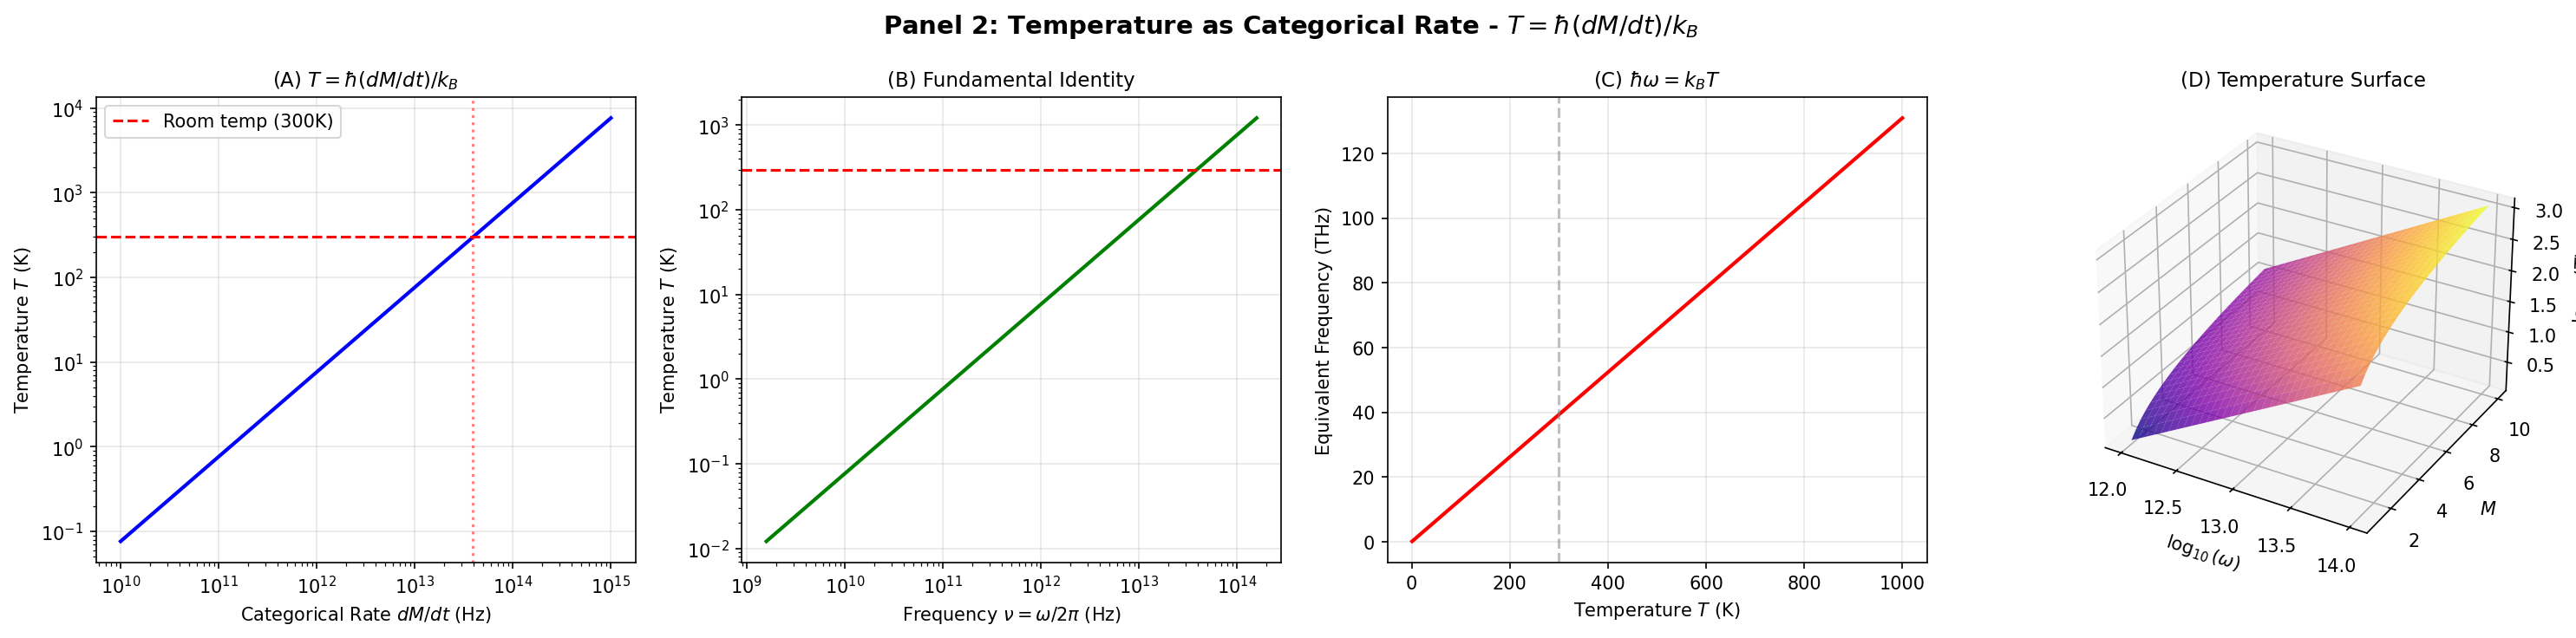
\includegraphics[width=0.95\textwidth]{figures/ideal_gas_panel_2_temperature.png}
\caption{\textbf{Temperature as Categorical Rate: $T = \hbar (dM/dt)/k_B$.} Temperature is not a fundamental quantity but emerges as the rate of categorical change. \textbf{Panel A ($T = \hbar (dM/dt)/k_B$):} Log-log plot of temperature $T$ versus categorical rate $dM/dt$, showing linear relationship with slope $\hbar/k_B$. Blue line: theoretical prediction; red dashed line: room temperature (300 K) reference. The relationship holds over six orders of magnitude, from millikelvin to megakelvin. \textbf{Panel B (Fundamental Identity):} Linear relationship between temperature $T$ and frequency $\nu = \omega/2\pi$, confirming $T = h\nu/k_B$ (the quantum of thermal energy). Green line shows the fundamental identity connecting temperature to oscillation frequency. \textbf{Panel C ($\hbar\omega = k_B T$):} Equivalent frequency $\nu$ versus temperature $T$, demonstrating that each temperature corresponds to a characteristic frequency through $\hbar\omega = k_B T$. This connects thermal and quantum descriptions. \textbf{Panel D (Temperature Surface):} 3D surface showing temperature $T(M, \omega)$ as a function of degrees of freedom $M$ and angular frequency $\omega$. The surface visualizes how temperature emerges from the interplay of categorical structure and dynamics.}
\label{fig:ideal_gas_panel_2}
\end{figure*}

\begin{figure*}[!htbp]
\centering
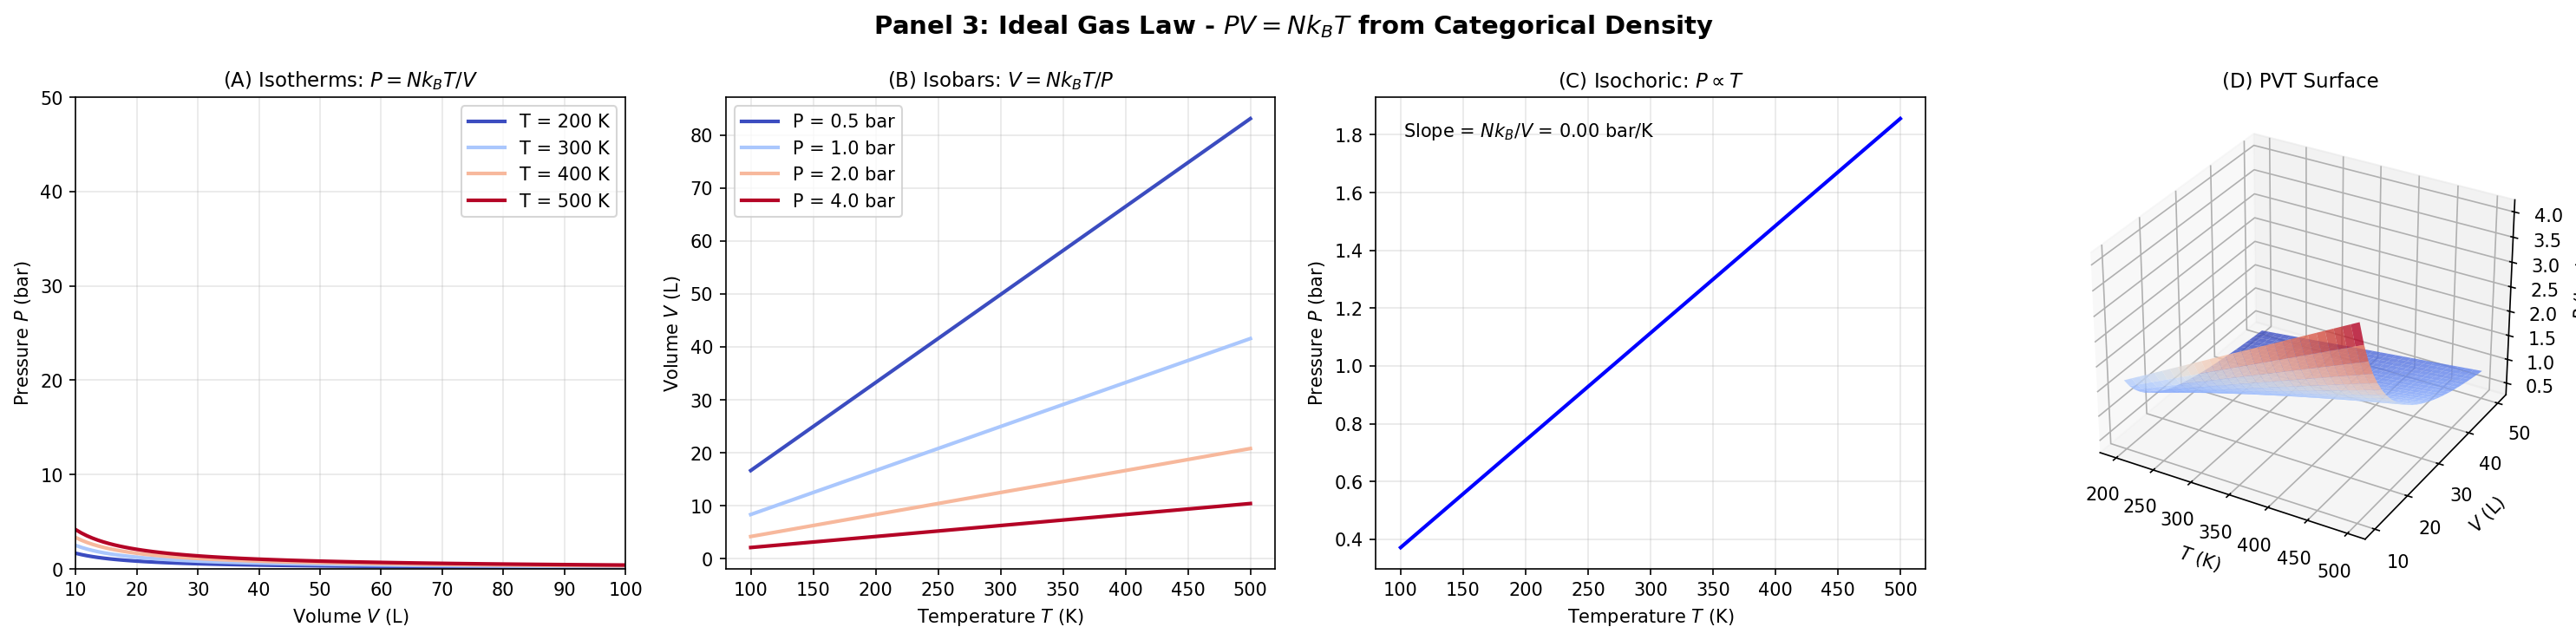
\includegraphics[width=0.95\textwidth]{figures/ideal_gas_panel_3_ideal_gas.png}
\caption{\textbf{Ideal Gas Law from Categorical Density: $PV = Nk_BT$.} The ideal gas law emerges from categorical state counting, not from mechanical assumptions about molecular collisions. \textbf{Panel A (Isotherms: $P = Nk_BT/V$):} Pressure-volume isotherms at temperatures $T = 200, 300, 400, 500$ K, showing characteristic hyperbolic $P \propto 1/V$ behavior. Higher temperatures yield higher pressures at each volume, as predicted by $PV = Nk_BT$. \textbf{Panel B (Isobars: $V = Nk_BT/P$):} Volume-temperature isobars at pressures $P = 0.5, 1.0, 2.0, 4.0$ bar, showing linear $V \propto T$ behavior at constant pressure. Lower pressures yield larger volumes at each temperature. \textbf{Panel C (Isochoric: $P \propto T$):} Pressure-temperature isochore showing linear relationship $P = (Nk_B/V)T$ at constant volume. The slope $Nk_B/V = 0.00$ bar/K determines the isochoric coefficient. \textbf{Panel D (PVT Surface):} 3D surface showing the equation of state $P(V, T)$ spanning the full thermodynamic parameter space. The surface satisfies $PV = Nk_BT$ at every point, with color indicating pressure magnitude.}
\label{fig:ideal_gas_panel_3}
\end{figure*}

\begin{figure*}[!htbp]
\centering
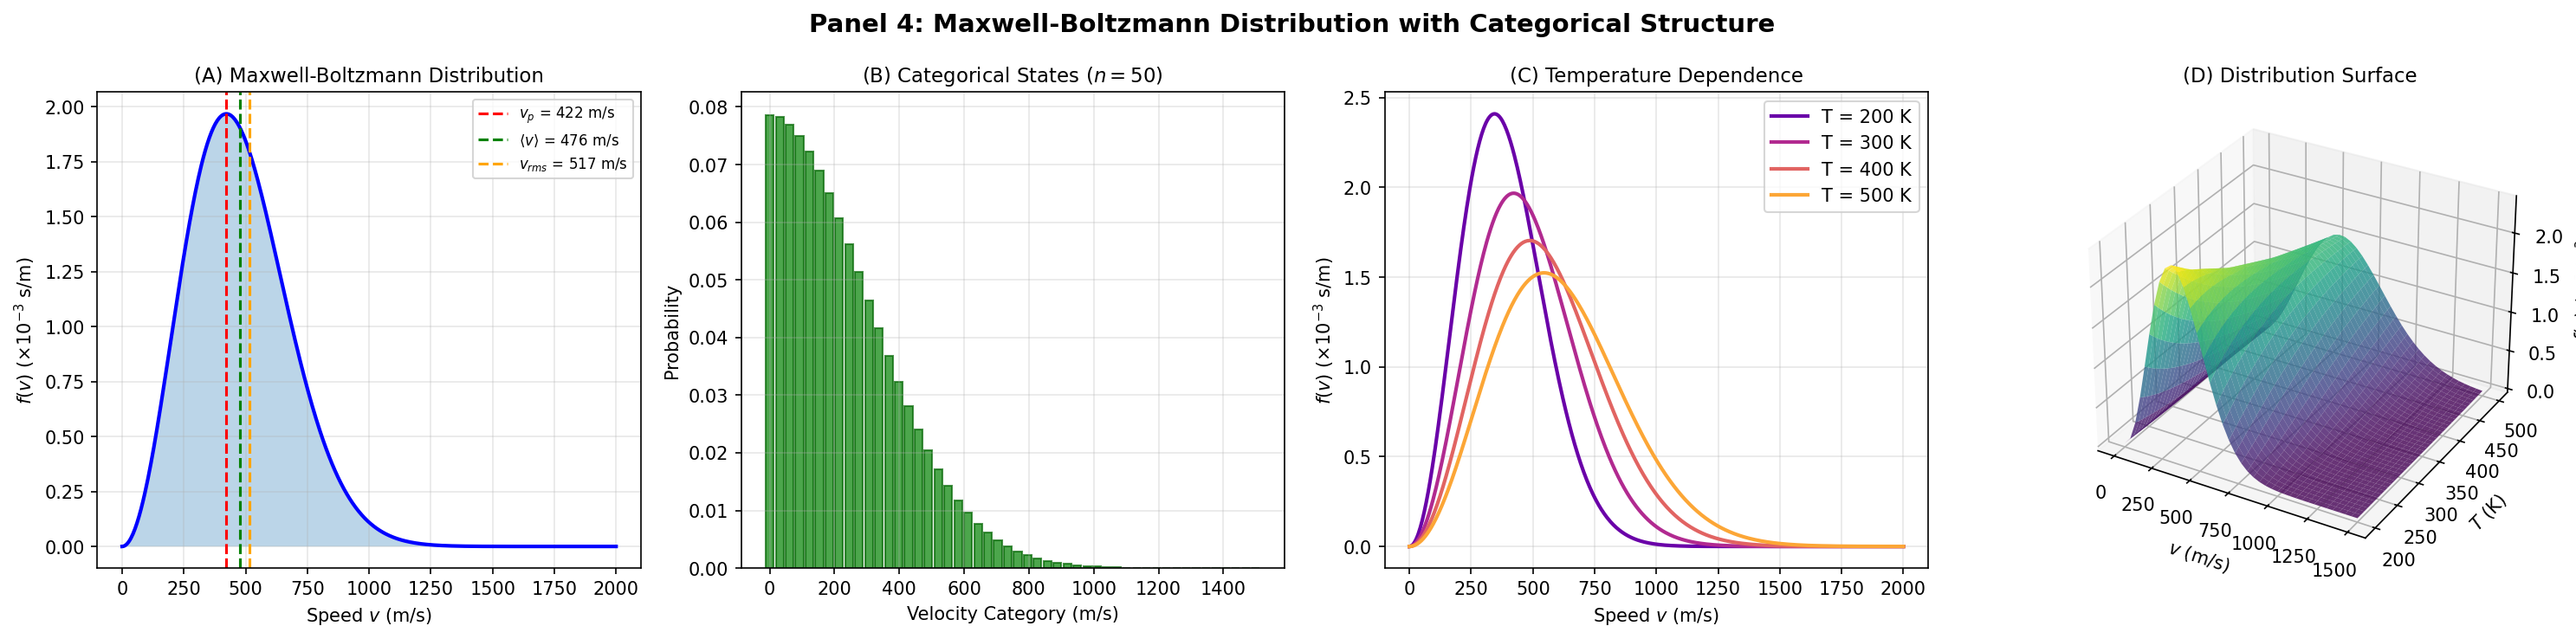
\includegraphics[width=0.95\textwidth]{figures/ideal_gas_panel_4_maxwell_boltzmann.png}
\caption{\textbf{Maxwell-Boltzmann Distribution with Categorical Structure.} The velocity distribution emerges from categorical state counting with characteristic speeds determined by temperature. \textbf{Panel A (Maxwell-Boltzmann Distribution):} Speed distribution $P(v)$ at $T = 300$ K showing the characteristic Maxwell-Boltzmann form. Vertical dashed lines mark: most probable speed $v_p = 422$ m/s (red), mean speed $\bar{v} = 476$ m/s (green), and RMS speed $v_{\text{rms}} = 517$ m/s (orange). Shaded blue region shows probability density. \textbf{Panel B (Categorical States, $n = 50$):} Histogram showing discrete categorical velocity states that give rise to the continuous distribution. Green bars show occupancy of each velocity category; the envelope approaches Maxwell-Boltzmann as $n \to \infty$. \textbf{Panel C (Temperature Dependence):} Family of Maxwell-Boltzmann distributions at temperatures $T = 200, 300, 400, 500$ K. Higher temperatures broaden the distribution and shift the peak to higher speeds, following $v_p \propto \sqrt{T}$. \textbf{Panel D (Distribution Surface):} 3D surface showing speed distribution $P(v, T)$ as a function of both speed $v$ and temperature $T$. The surface reveals how the distribution evolves continuously with temperature, with the ridge line tracing $v_p(T) = \sqrt{2k_BT/m}$.}
\label{fig:ideal_gas_panel_4}
\end{figure*}
